%  Robotics Text  by Jacob Rosen and Blake Hannaford
% (c) 2007  Jacob Rosen and Blake Hannaford
%

\chapter{Differential Kinematics - The Jacobian Matrix}

\section{Problem Statement and Learning Objectives}
% Problem Statement and Learning Objectives for Chapter 05

\paragraph{Problem Statement}
 
\paragraph{Learning Objectives}
Upon completing this Chapter, the reader should be able to
\begin{itemize}
  \item compute velocity with different frames of computation and representation and understand the difference between these two frames. 

  \item define the linear and angular velocity of a rigid body. 

  \item compute the velocity and angular velocity of a link, based on the DH parameters and the velocities of the previous link.

  \item propagate the velocity calculation down the serial link chain to compute linear and angular velocity of an end effector. 

  \item extract a Jacobian Matrix from the velocity propagation calculation. 

  \item  state the relationship between joint velocities and end effector velocities using the Jacobian Matrix. 

  \item state the relationship between joint torques and end effector forces using the Jacobian Matrix. 
\end{itemize}


\section{Velocity}

\subsection{Velocity and Acceleration of a Particle}

Velocity is based on a differential measurement or calculation of position, $\Delta X = X(t+\Delta t) - X(t)$. In order for this subtraction to be valid, both $X(t+\Delta t)$ and $X(t)$ must be represented in the same frame which we will call the {\it computation frame}.   If this frame is moving, we might get a very different result from use of a fixed frame. This is not a bad thing however.  Depending on our needs, either a moving or fixed frame might be preferable.   Another part of the velocity computation is dividing by $\Delta t$, but $\Delta t$ is a scalar, and thus is the same in every frame (leaving out relativistic effects!).

The second key frame is the frame in which we represent the velocity after it is computed, the {\it representation frame}.   Once we have
$\frac{\Delta X}{\Delta T}$, we have a free vector, and this may be transformed (by rotation) into any frame we desire.  This second frame is called the representation frame.


%  Table row height
\renewcommand\arraystretch{0.2}% Vertical Row size, 1.0 is for standard spacing)


%\begin{slide}
%%%%** Section 1
\paragraph{Velocity of a Vector}
If $^AQ$ is a point represented in frame $A$, then
\[
^AV_Q = \lim_{\Delta t \to 0} \left( \frac{
     ^AQ(t+\Delta t) - {^AQ}(t)}
     {\Delta t} \right)
\]
We have just {\it computed} the velocity in frame $A$ and it is also {\it represented}
in frame $A$.

Later we may wish to  represent the velocity in another frame
e.g.:
\[
^B(^AV_Q) = {^B_AR} {^AV_Q}
\]
If we use the notation:
\[
^A(^BV_P)
\]
We mean\\
$A$ is the {\it representation} frame. \\
$B$ is the {\it computation} frame. \\
$P$ is the point whos velocity we are talking about.

If a velocity is computed and represented in the same frame, we use just one
superscript:
\[
^A(^AV_P) \to ^AV_P
\]


\begin{Example}
To illustrate the difference between {\it computation} and {\it representation}
of velocity vectors, consider the following example.   A car is driving along a road.
Its speedometer reads a constant 55 mph.  The road is divided into four regions according to the map below.

\vspace{0.15in}
\begin{center}
\scalebox{0.2}{
   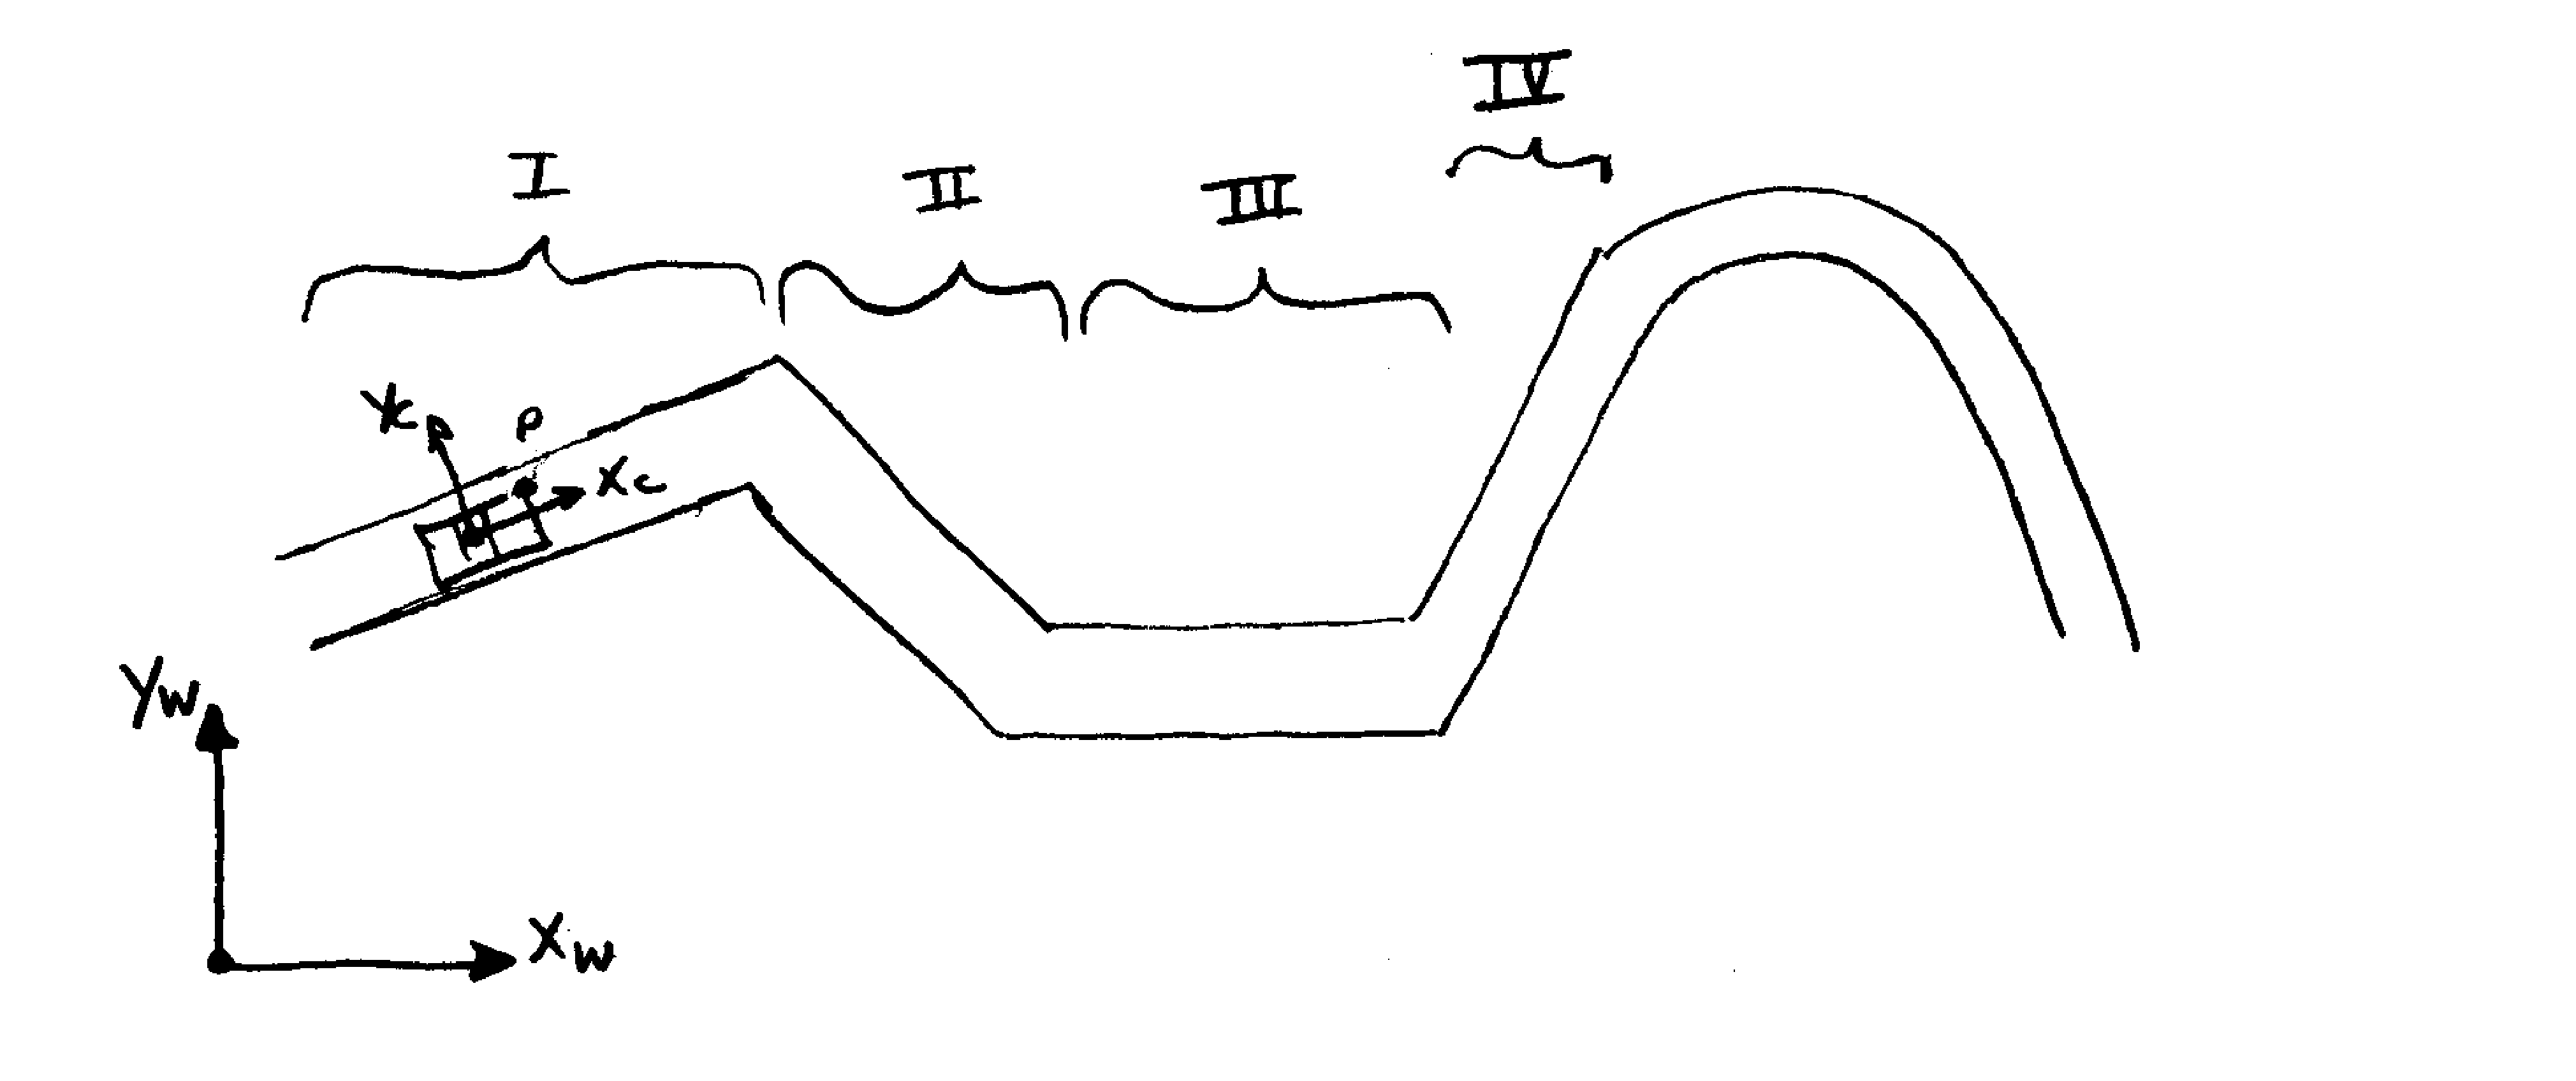
\includegraphics{figs05/00229.eps}
   }
\end{center}

$C$ is a frame fixed to the car.  $W$ is a frame fixed to the earth.  $P$ is a point on the car.

What are some different velocity vectors for each of the regions I ... IV?

\[
^C(^CV_P) = \left [
\begin{array}{c}
0 \\
0 \\
0 \\
\end{array}
\right ]
\]
In this example, the velocity of point, $P$ is computed in the Car frame and represented in the car frame.   However since $P$ is a fixed point on the car, it's velocity in the car frame is zero.  In fact this is true for all regions of the map.
Also, note that
\[
^W(^CV_P) =
\left [
\begin{array}{c}
0 \\
0 \\
0 \\
\end{array}
\right ]
\]

Why? Because if we rotate this velocity, it's still zero.

\[
^C(^WV_P) =  \left [
\begin{array}{c}
55mph \\
0 \\
0 \\
\end{array}
\right ]
\]
In this example, the velocity of $P$ is computed in the world frame.   This must have a magnitude of 55mph and it must point in the positive $X_C$ direction because we assume the car is going in forward gear!  Since the velocity is represented in the car frame, it must be constant and independent of the region.

Supposed we are asked to diagram
$
^W(^WV_P)
$
on the coordinate system $\{X_W,Y_W\}$:  What would that look like?\\[0.15in]

\scalebox{0.2}{
  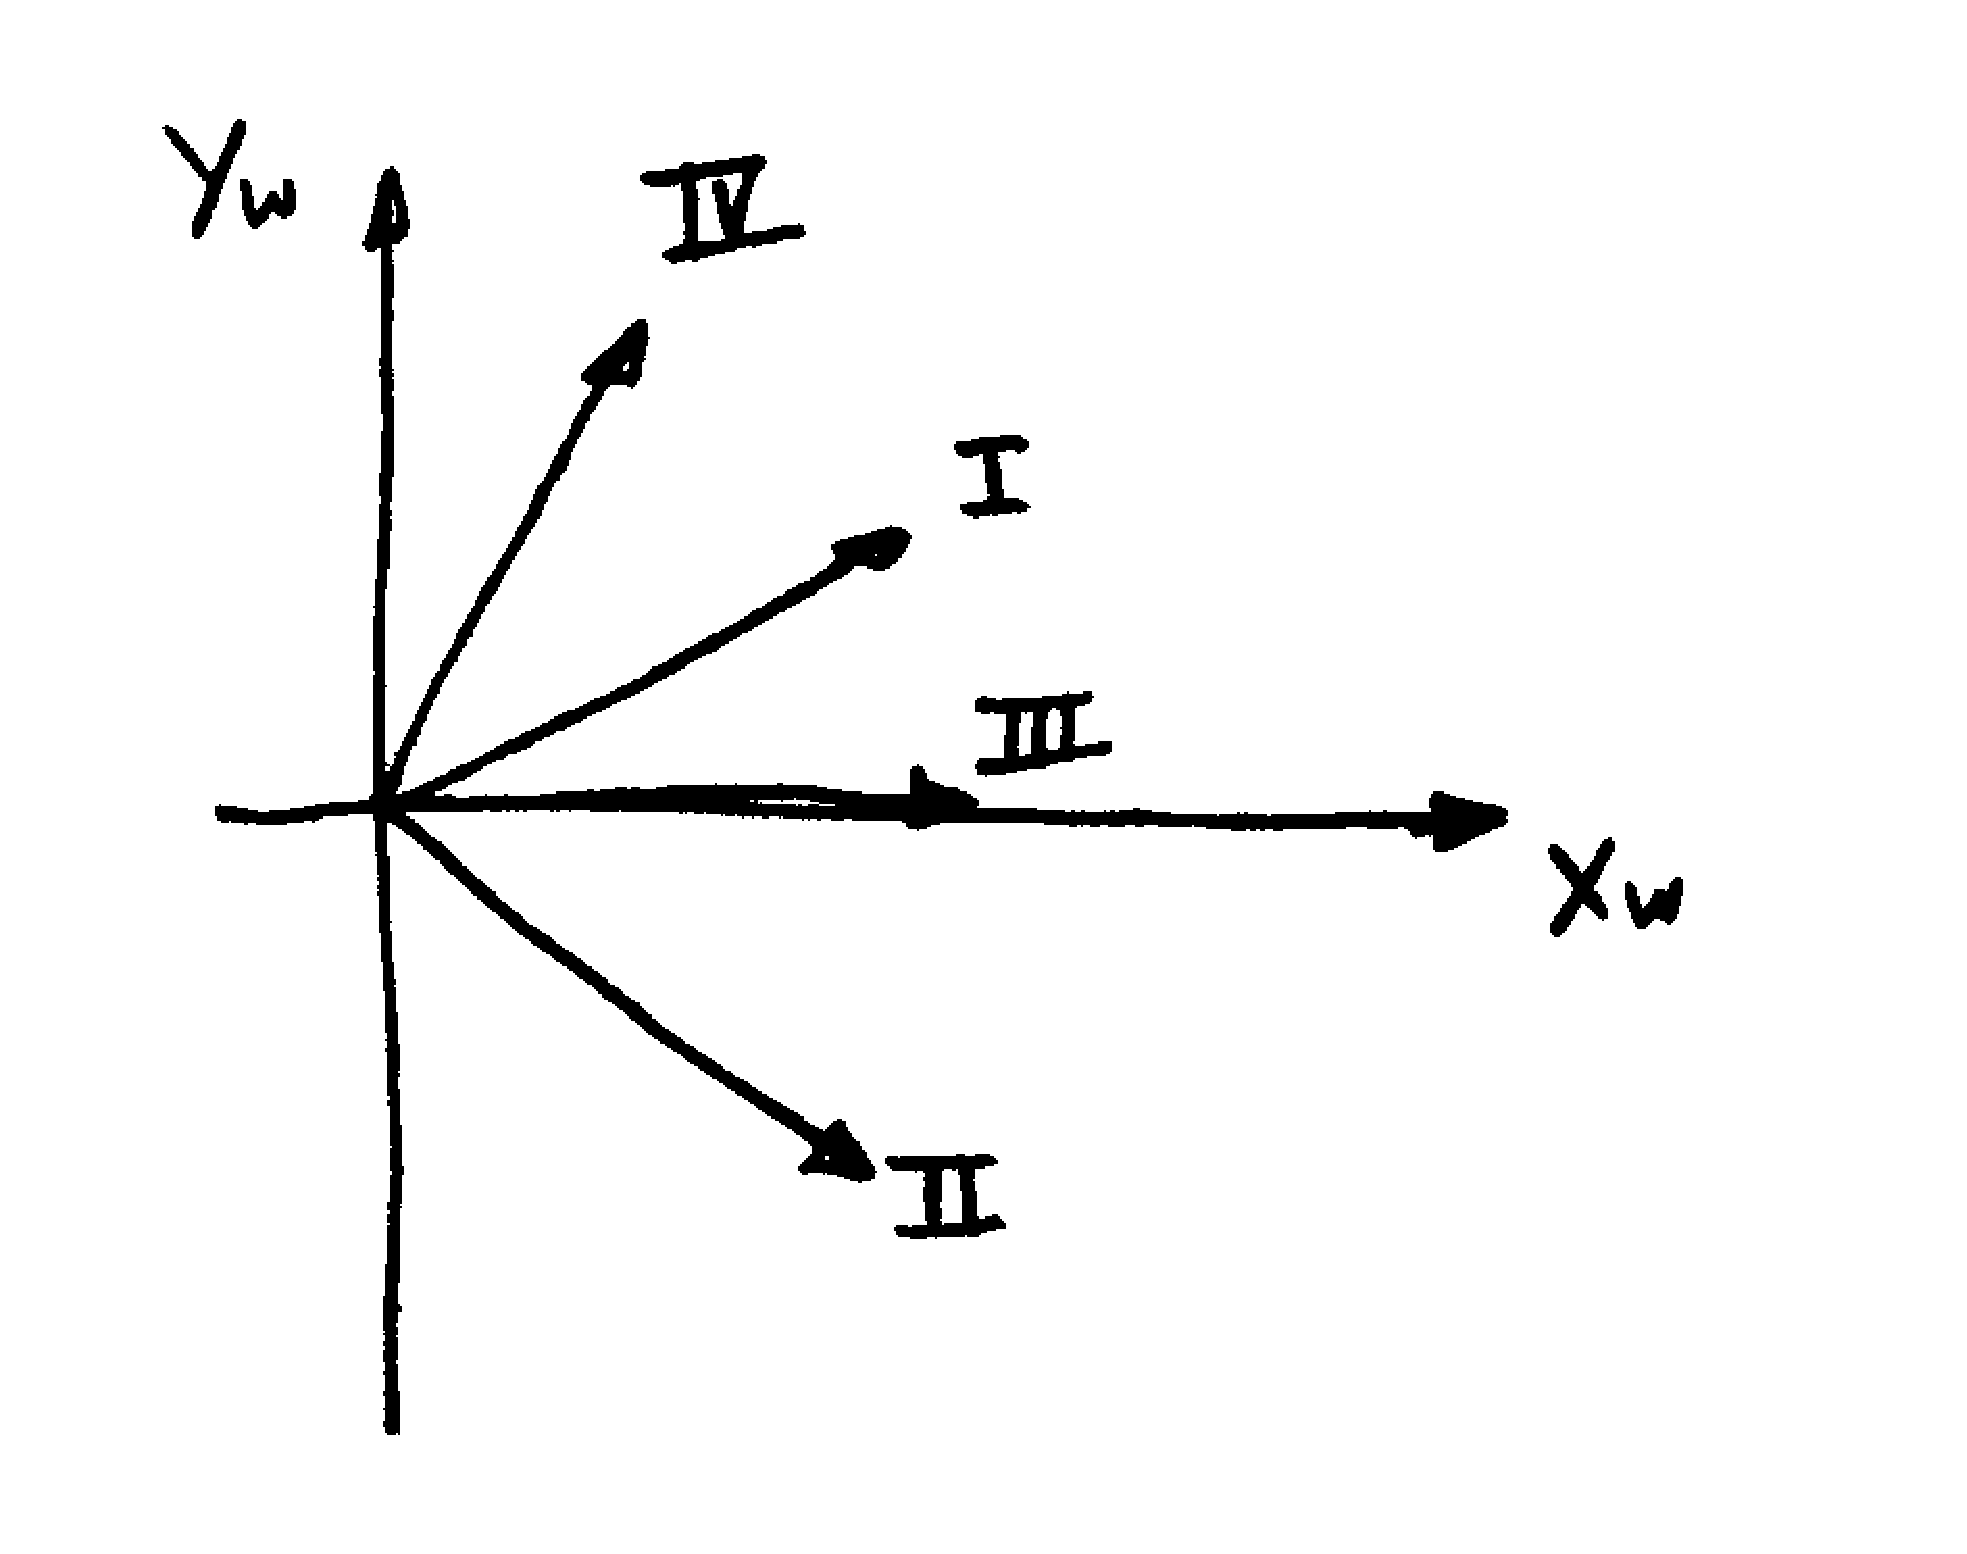
\includegraphics{figs05/00231.eps}
  }

We know $|^W(^WV_P)| = 55mph$ since the speed is a constant 55.  Only the direction in frame $W$ changes in each region.



%       Blank Solutions
%
%\[
%^C(^CV_P) = \left [
%\begin{array}{c}
%? \\
%? \\
%? \\
%\end{array}
%\right ]
%\]
%(what is the answer for regions I,II,III,IV?)
%
%\[
%^C(^WV_P) =  \left [
%\begin{array}{c}
%? \\
%? \\
%? \\
%\end{array}
%\right ]
%\]
%
%\[
%|^W(^WV_P)| = ?
%\]
%
%Diagram:
%$
%^W(^WV_P)
%$
%On the coordinates:\\
%
%\scalebox{0.2}{
%  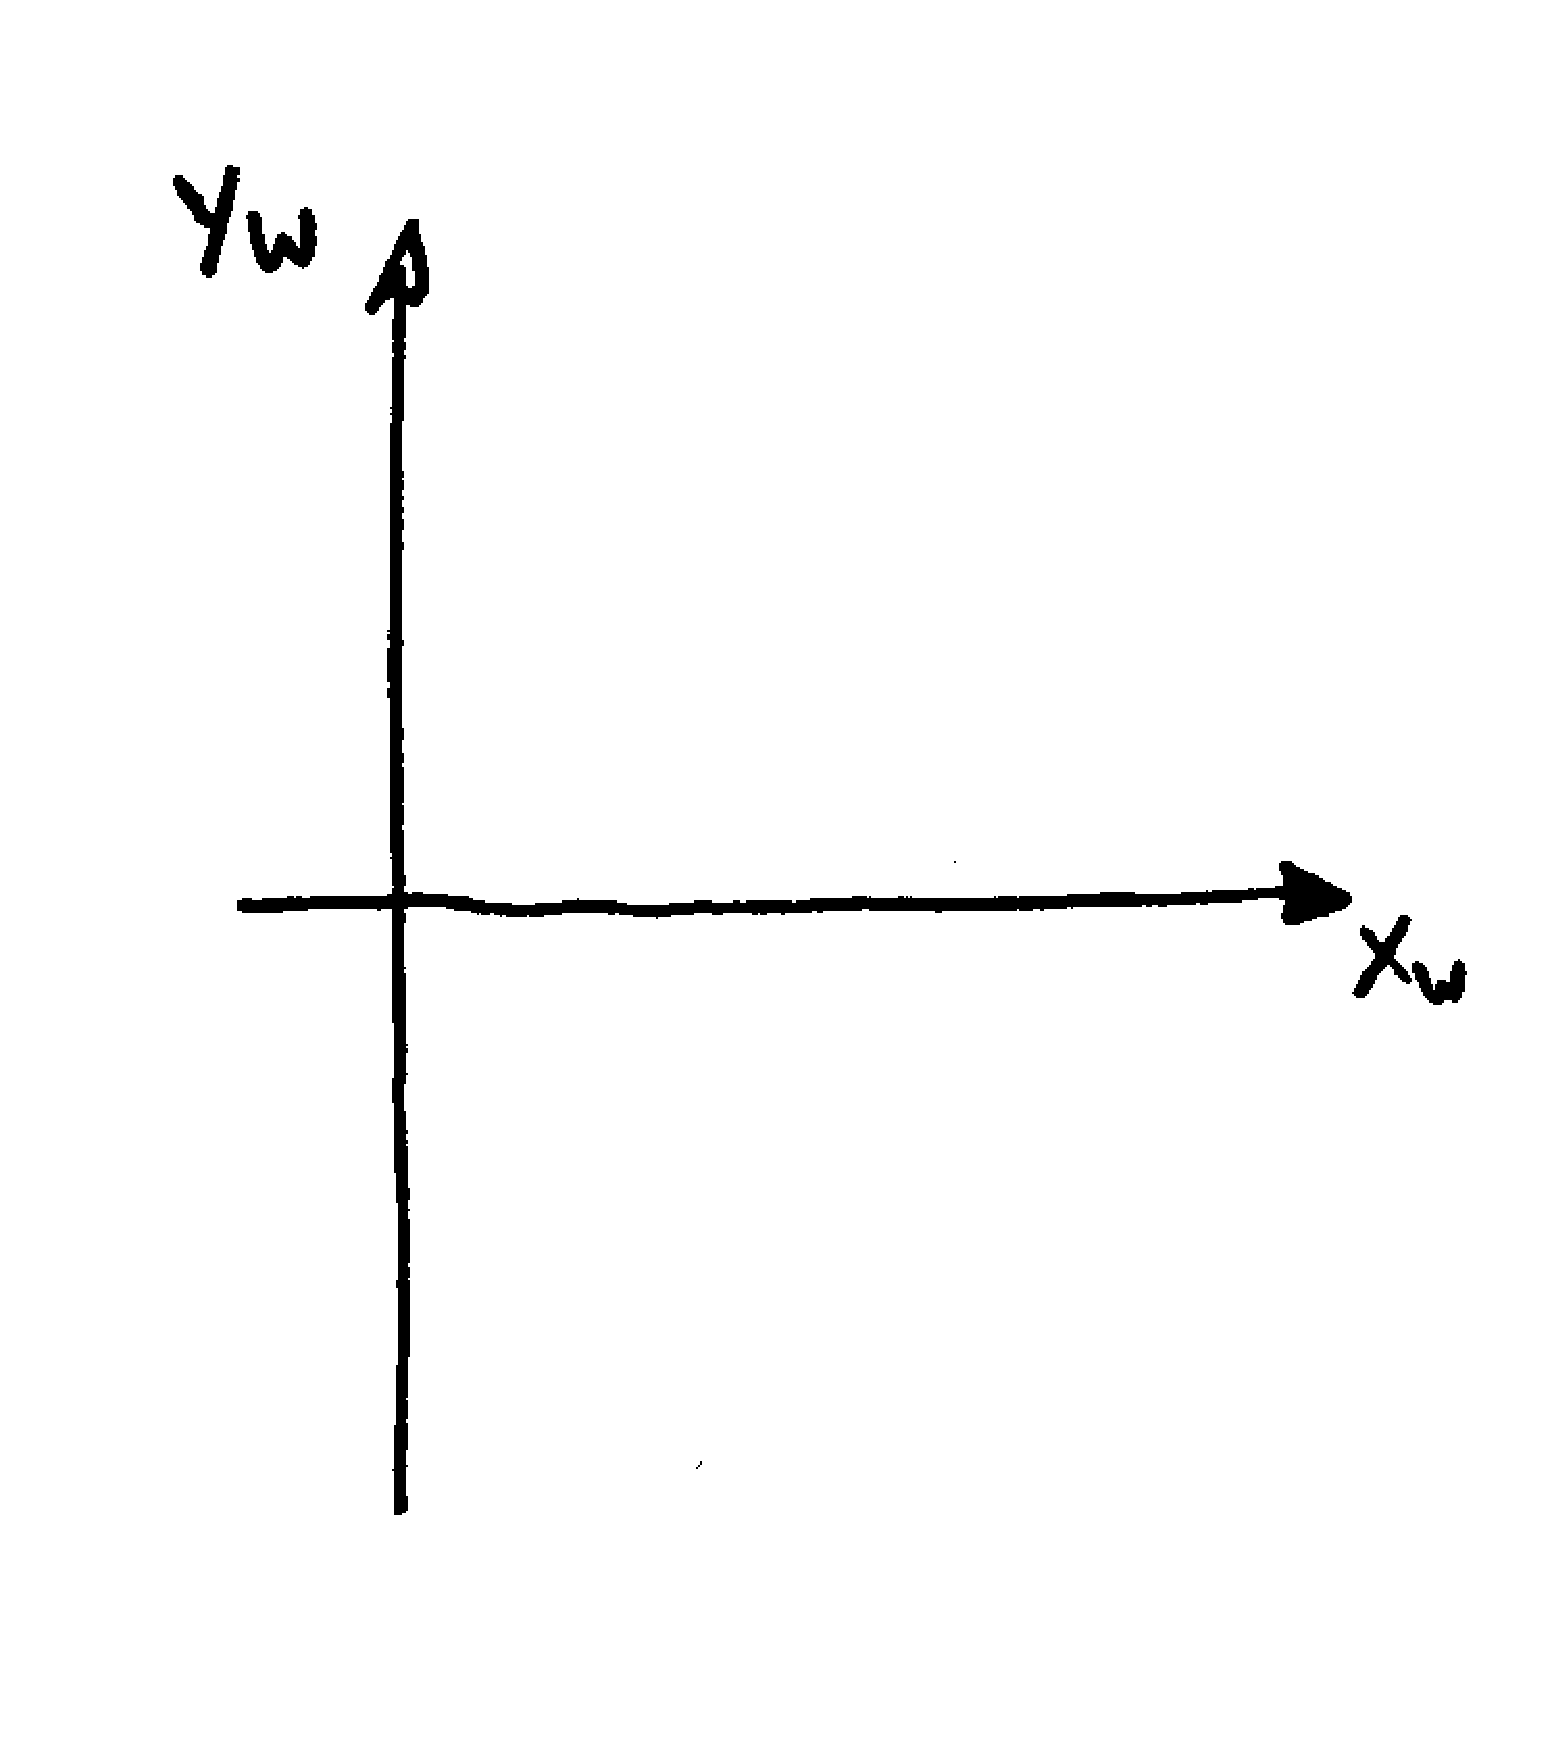
\includegraphics{figs05/00230.eps}
%  }
	%<*>

\end{Example}




\subsection{Rigid Bodies and Angular Velocity}\label{sectionrigidbodies}

Going beyond velocity of single points requires us to consider rigid bodies.
Rigid bodies can be thought of as a collection of points, all of which have a fixed location in a frame called an object frame.   A rigid body has two types of velocity: linear (translational) velocity which describes its rate and direction of translation, and angular velocity which describes its rotation.

\paragraph{Linear Velocity}  Linear velocity of a rigid body is represented the same as velocity of a point, having a computation frame and a representation frame.   However, nonzero angular velocity of an object will cause each point in the object to have a different linear velocity.

\paragraph{Angular Velocity}
Angular velocity can be   understood through the following properties
\begin{itemize}
  \item Angular velocity, $\Omega$, is a vector whos direction is the axis
  of rotation and whos magnitude is the rate of rotation, $\omega$.

  \item If a point is displaced from the axis of rotation, that point will
  have a linear velocity component corresponding to the rotation:
  \[
    V = \Omega \otimes r
  \]
  where $r$ is a vector from a point on the axis of rotation to the point.

  \item The vector cross product $\otimes$ can be defined as
  \[
  A = B \otimes C
  \]
  \[
  |A| = |B||C|\sin\theta
  \]
  \[
  A \bot B,  A\bot C
  \]
  where $\theta$ is the angle between the two vectors
  by the Right Hand Rule.

  \item Another way to compute $\otimes$ is using a skew symmetric matrix:
If $a$ and $b$ are 3 dimensional vectors,
\[
a \otimes b = \left[ \begin{array}{ccc}
0 & -a_3 & a_2 \\
a_3 & 0 & -a_1 \\
-a_2 & a_1 & 0
\end{array} \right]
\left[ \begin{array}{c}
b_1 \\
b_2 \\
b_3
\end{array} \right]
\]

  \item The angular velocity of a rigid object is the same for all
  points in that object.

\end{itemize}




\paragraph{Angular Velocity Generates Linear Velocity}

In this section we consider the effects of velocity on different parts of
 an object or robot arising from the second point above.

First, consider a rigid object with a frame, $O$, attached to it (Figure \ref{rigidbodyvelocities}).

\begin{figure}\centering
   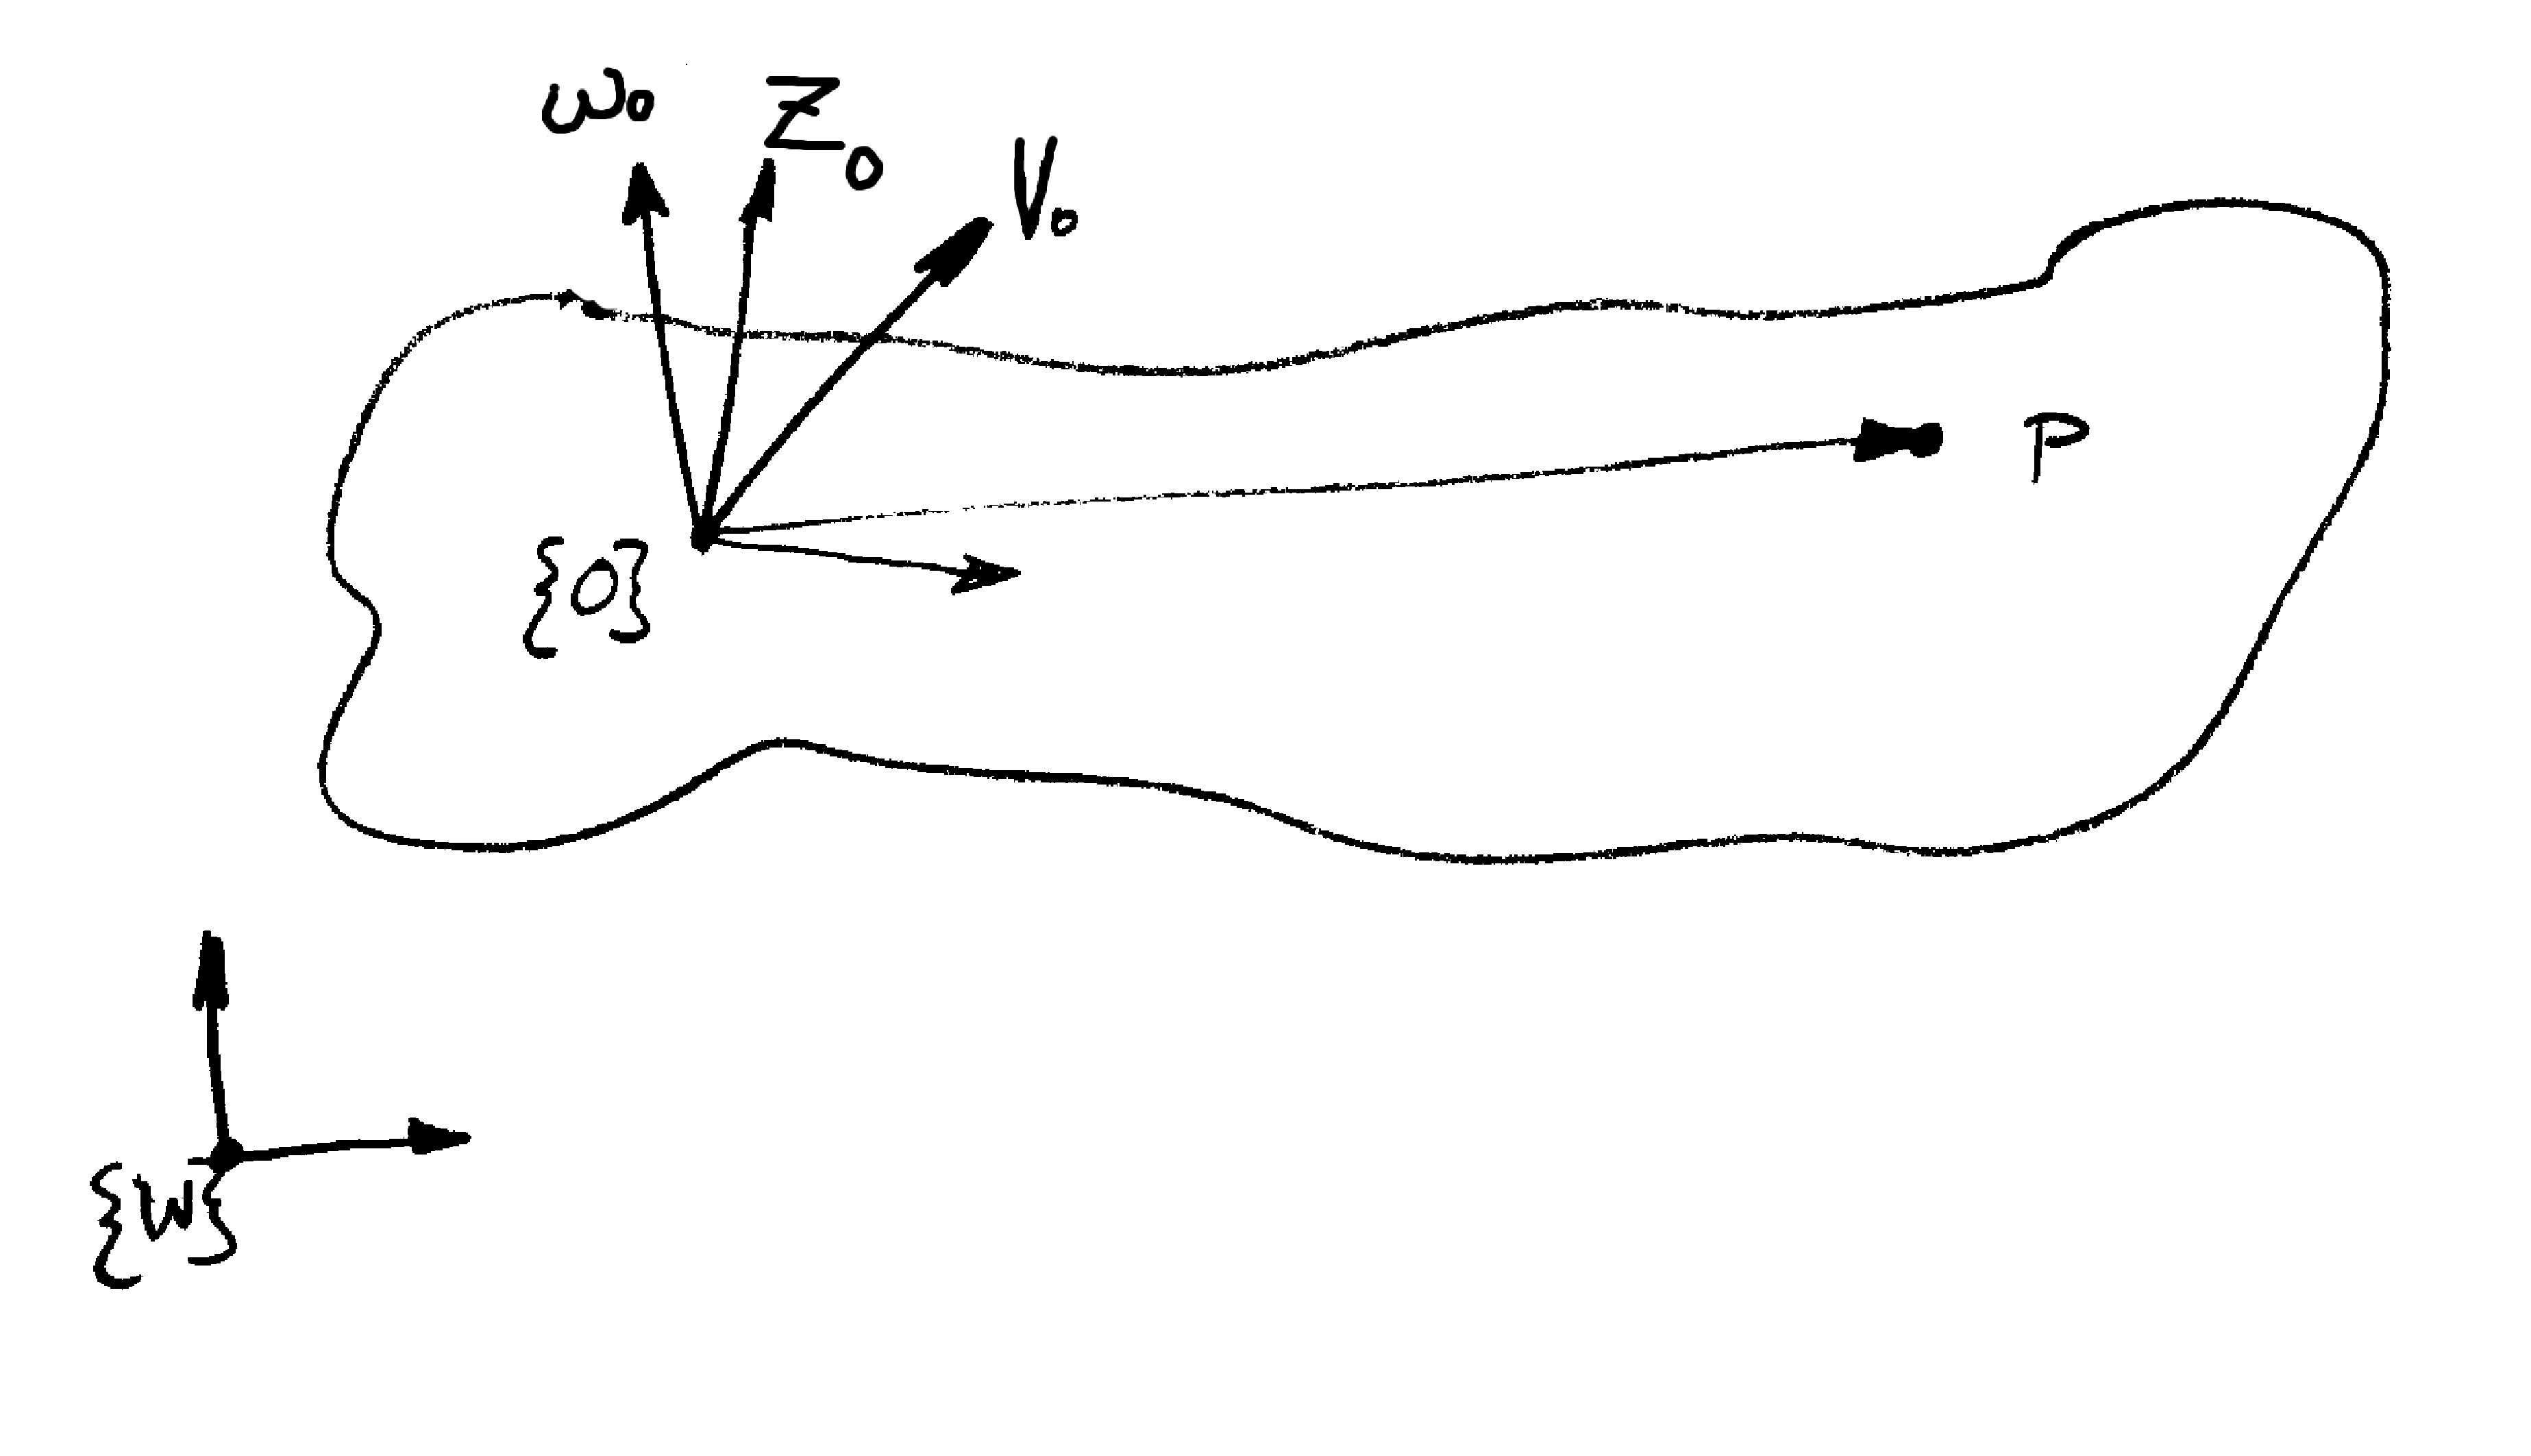
\includegraphics[width=85mm]{figs05/00064.eps}
   \includegraphics[width=85mm]{figs05/00707.eps}
\caption{Velocity of any point on a rigid object can be computed from it's location in the object frame, using the linear and angular velocity of the body (also represented in the object frame).}\label{rigidbodyvelocities}
\end{figure}

The origin of frame 0, \{O\},  has velocity $V_O$ and the object has angular velocity
$\omega_O$ which are computed in the world frame, $W$, and represented in {\it any}
frame.
What is the velocity of a point, $P$, on the object?

The answer has two components
\begin{itemize}
  \item The velocity of the object, $V_O$.
  \item Additional velocity due to the rotation of the object: $ V = \omega_O\otimes P$
\end{itemize}

So its total velocity is
\[
^*(^WV_P) = V_O + \omega_O\otimes P
\]
Where the * is meant to indicate that this equation is true in any frame,
so long as all terms are represented in that same frame.




% ///////////////////////////////////////////////////////////////////////////////////////////////////////////////////
% /////////
% //    New quaternion material for velocity
% //

\subsection{Quaternions and Angular Velocity}

Quaternion representation of orientation (Section \ref{QuaternionSection})  can also be differentiated and related to angular velocity.  First, we define the notion of the time derivative of a quaternion\footnote{\small\tt http://www.euclideanspace.com/physics/kinematics/angularvelocity/}.

Differentiating equation \ref{quaterniondefinition}
\[
\frac{dq}{dt} =  \frac{1}{2} \dot{\theta} \left [ -\sin(\theta/2) + K_xi\cos(\theta/2)+K_yj\cos(\theta/2)+K_zk\cos(\theta/2) \right]
\]

then it can be derived that

\[
\begin{bmatrix} 0 \\ \omega_x \\ \omega_y \\ \omega_z \end{bmatrix} = 2\frac{dq}{dt}q^*
\]
where $q^*$ is the inverse of $q$ (equation \ref{quaternioninversedefinition}).

If the angular velocity $\omega$ is known, then $\frac{dq}{dt}$ is
\[
\frac{dq}{dt} = 1/2 \begin{bmatrix} 0 \\ \omega_x \\ \omega_y \\ \omega_z \end{bmatrix} q
\]
.




\section{The Jacobian Matrix}
\subsection{Velocity Mapping}
In the forward kinematics model, we saw that it was possible to relate joint angles, $\theta$, to the configuration of the robot end effector, $^0_6T$. In this chapter we will work on the relationship between the joint rates, $\dot{\theta}$, and the velocity of the end effector, $\dot{x}$ with a matrix as follows:
\[
\dot{x} = J(\theta)\dot{\theta}
\]
Here the velocity $\dot{x}$ describes both linear and rotational components.   An expanded version of the previous equation is
\[
\left [ \begin{array}{c}  \dot{x} \\[5pt]  \dot{y} \\[5pt] \dot{z} \\[5pt]
                          \omega_x \\[5pt] \omega_y \\[5pt] \omega_z
\end{array}  \right ]
=
\left [  \begin{array}{cccc}
 & & & \\
 & & & \\
 & & J(\theta) & \\
 & & & \\
 & & & \\
 & & & \\
\end{array} \right ]
\left [  \begin{array}{c}
\dot{\theta_1} \\[5pt]
\dot{\theta_2} \\[12pt]
\dots          \\[12pt]
\dot{\theta_N} \\[5pt]
\end{array} \right ]
\]

$\omega_i$ are the components of angular velocity, and $J(\theta)$ is a matrix of size 6x$N$ where $N$ is the number of joints in the robot. We will derive $J(\theta)$ by calculating $\dot{x}$ as a function of $\dot{\theta}$ and factoring out $J(\theta)$.  But first, as a simple illustration let us consider a   planar example:

\begin{Example}
Compute the velocity of the end effector of this basic planar robot as a function of its joint velocity $\dot{\theta}$.

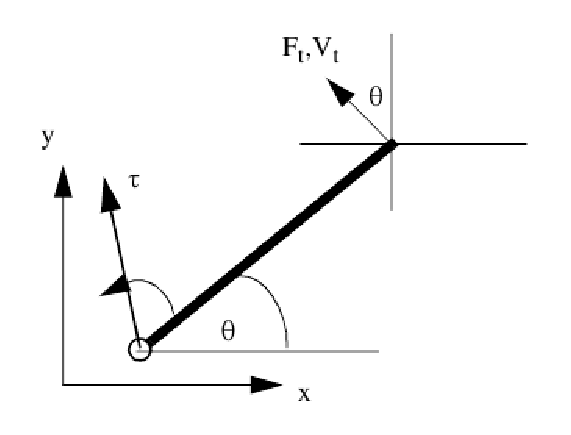
\includegraphics[width=3.0in]{figs05/planar_examp.eps}

Looking at the figure, we can resolve the velocity of the tip into x and y components as follows:
\[
v_x = -r\dot{\theta}\sin(\theta)  \qquad   v_y = r\dot{\theta}\cos(\theta)
\]
This can be expressed as a trivial matrix equation as follows:
\[
\left [ \begin{array}{c}
v_x \\ v_y
\end{array} \right ]
=
\left [ \begin{array}{c}
-r\sin(\theta) \\ r\cos(\theta)
\end{array} \right ]
\dot{\theta}
\]
or
\[
J(\theta) =
\left [ \begin{array}{c}
-r\sin(\theta) \\ r\cos(\theta)
\end{array} \right ]
\]

\end{Example}


This chapter will cover the Jacobian Matrix and how to compute it in detail, but first we want to give
the bird's eye view of this powerful matrix.  This section aims to show what kinds of problems
we can solve once we solve the Jacobian Matrix.


%%%%** Section 2
\paragraph{Spaces}

Consider three spaces relevent to robot arm motion (Figure \ref{Spaces}).

\begin{itemize}
\item Joint Space\\
A point in this space is located by the values of the $N$ joint variables of the arm.
\item Configuration Space\\
A point in this space is located by the $X,Y,Z$ position of the end effector plus three rotation variables which describe its orientation such as roll, pitch, yaw angles.
\item Cartesian Task Space\\
A point in this space is determined by $X,Y,Z$.  The configuration of a rigid object in Cartesian task space is defined by its $4\times4$ homogeneous transform.
\end{itemize}



%%%%** Figure 1
\begin{figure}[h]
\centering
\scalebox{0.2}{
   \includegraphics{figs05/00225.eps}
   }
\caption{Three spaces relevent to robot arm motion: Task space, Joint Space, Configuration Space.}\label{Spaces}
\end{figure}

In Chapters 2 and 3, we've seen the static mappings between Joint Space and Cartesian Task Space,  the Forward Kinematic
Mapping (Fkin) and the Inverse Kinematic Mapping (Kin$^{-1}$) (Figure \ref{Static}).

%%%%** Figure 2
\begin{figure}[h]
\centering
\scalebox{0.2}{
  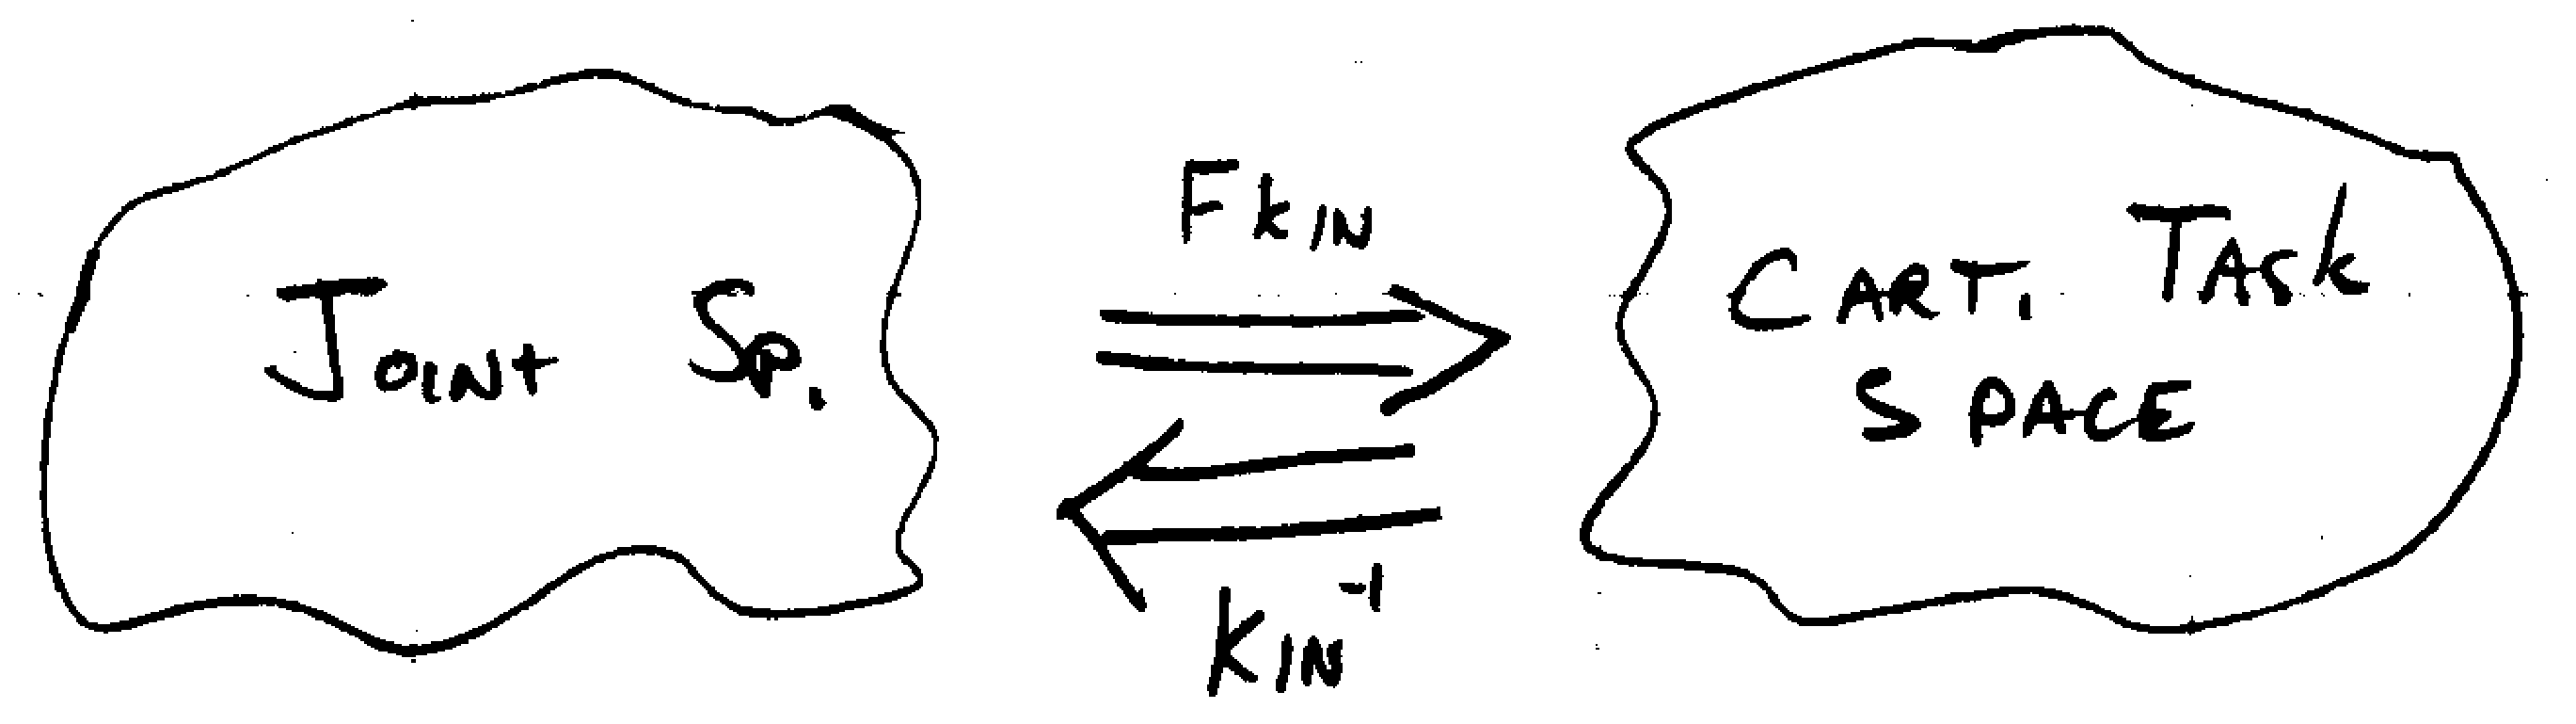
\includegraphics{figs05/00228.eps}
   }
\caption{Static mappings between Joint space and Cartesian Task Space.}\label{Static}
\end{figure}

Now we introduce {\it incremental} mappings between small changes in joint space and small changes
in task space. i.e.
\[
\Delta X = J(\theta)\Delta \theta
\]
\[
\dot{x} = J(\theta)\dot{\theta}
\]
and
\[
\dot{\theta} = J^{-1}(\theta)\dot{x}
\]


%%%%** Figure 3
\begin{figure}[h]
\centering
\scalebox{0.2}{
   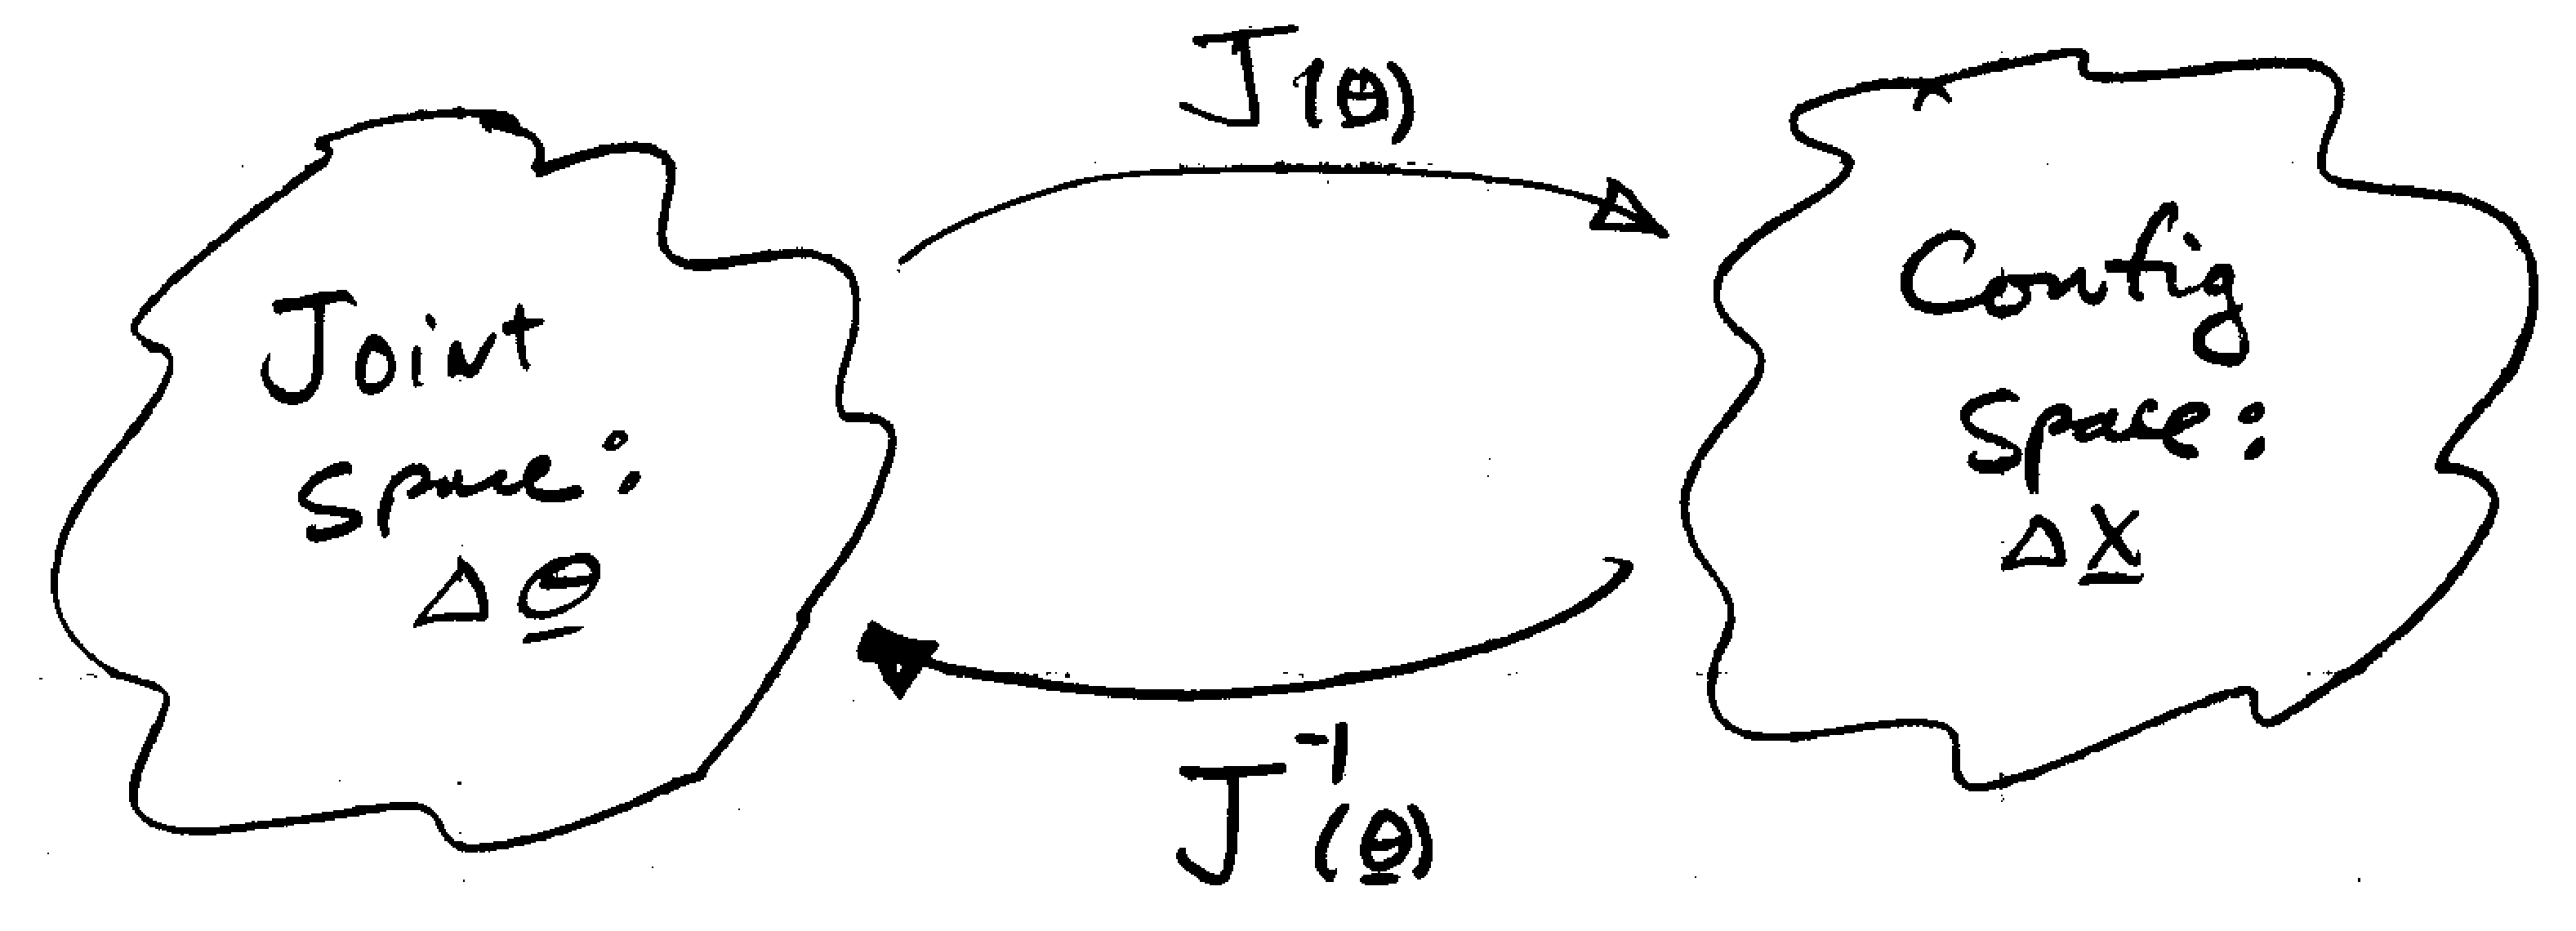
\includegraphics{figs05/00226.eps}
   }
\caption{Incremental Mapping between spaces}\label{IncSpaces}
\end{figure}


We can apply these mappings to answer several interesting questions:

%%%%** Section 2.1
\paragraph{Velocity Mapping}

\noindent
{\bf Q:}  What velocity and angular velocity will be generated at the tip
of the robot if all joints are driven at 0.1 rad/sec?

\noindent
{\bf A:}
\[
\dot{x} = J(\theta)
\left [
\begin{array}{c}
0.1 \\[6pt]
0.1 \\[6pt]
 \\[12pt]
\dots \\[12pt]
 \\[6pt]
0.1 \\
\end{array}
\right ]
\]
note that this solution is a function of $\theta$.

\noindent
{\bf Q:} How should we drive the joints so that the end effector tracks a target
moving with velocity
\[
\dot{x}_t =
\left [
\begin{array}{c}
1\\[6pt]
0\\[6pt]
0.5\\[6pt]
0\\[6pt]
0\\[6pt]
0\\[6pt]
\end{array}
\right ]
\]

\noindent
{\bf A:}
\[
\dot{\theta} = J^{-1}(\theta)
\left [
\begin{array}{c}
1\\[6pt]
0\\[6pt]
0.5\\[6pt]
0\\[6pt]
0\\[6pt]
0\\[6pt]
\end{array}
\right ]
\]

notes:  Does $J(\theta)^{-1}$ exist?  What about `conditioning' of $J(\theta)$?

%%%%** Section 2.2
\subsection{Force Mapping}

\begin{ExampleCont}
Referring back to the single-joint arm of this example,
we can look at the tip force, and the torque around the joint:
\[
\tau = -r F_x\sin(\theta)+rF_y\cos(\theta)
\]
This again gives a trivial matrix equation:
\[
\tau =
\left [ \begin{array}{cc}
-r\sin(\theta) & r\cos(\theta)
\end{array} \right ]
\left [ \begin{array}{c}
F_x \\ F_y
\end{array} \right ]
\]
Note that the first term happens to be the transpose of the matrix $J(\theta)$ computed above.  As we will show below, this is $not$ a coincidence, so we can write
\[
\tau = J^T(\theta) F
\]
\end{ExampleCont}

Thus when mapping Forces and Torques between the same spaces:
\[
\tau = {J(\theta)}^T F
\]
\[
F = {J(\theta)}^{-T}\tau
\]

Notes:
\begin{enumerate}
\item  ${J(\theta)}^{-T}$ indicates the inverse of $J(\theta)^T$.
\item Mappings are a function of $\theta$.
\item Does ${J(\theta)}^{-T}$ exist?
\end{enumerate}


%%%%** Figure 4
\begin{figure}
\centering
\scalebox{0.2}{
  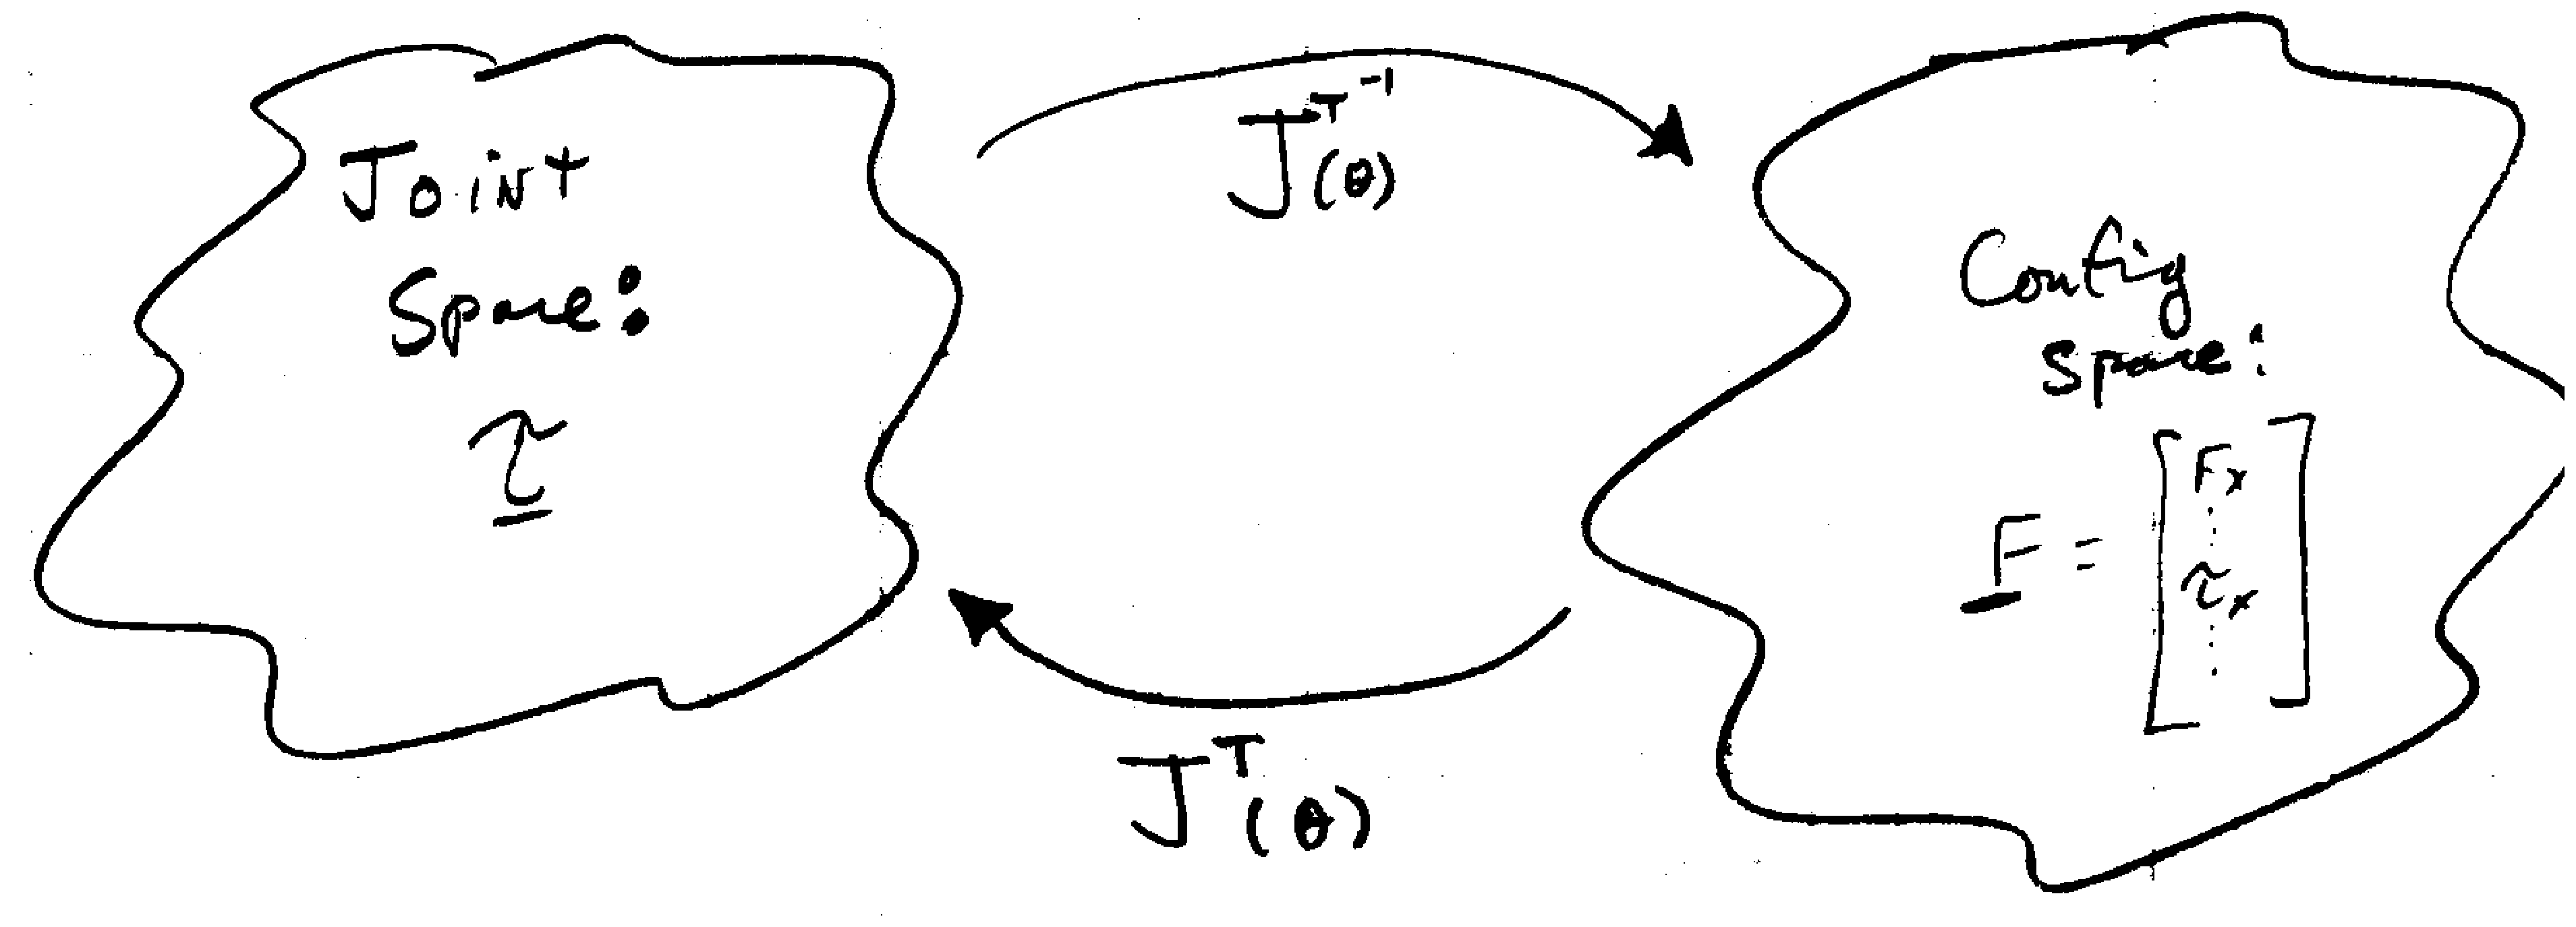
\includegraphics{figs05/00227.eps}
   }
\caption{Mappings between joint torques and end effector forces.}\label{FSpaces}
\end{figure}






\subsection{Virtual Work}

It's not obvious that the Jacobian matrix should relate {\it both} incremental motions and also forces and torques between the joint space and configuration space.
The concept of virtual work can be used to derive the force and torque mapping role of the
Jacobian Matrix from its incremental motion mapping role.


We consider the mechanism to be purely kinematic. This means that it has
no ability to dissipate or  store energy:
\begin{itemize}
\item no friction (energy loss)
\item no inertia (kinetic energy)
\item no mass (potential energy due to gravity)
\item no compliance (potential energy due to elastic energy of deformation)
\end{itemize}
These assumptions might seem quite unrealistic.  In fact many robot motions involve low enough amounts of energy that the assumptions are quite useful.

Let's review some definitions:

\begin{description}
\item[Power] $P = \frac{d}{dt}E$ (where $E$ is energy)
\item[Power] $P = F \cdot V = F^TV$
\item[Power] $P = \tau \cdot \omega = \tau^T\omega$
\item[Work] $W = \Delta E = P\Delta t$
\end{description}

Because of the properties above, if we apply some work to part of the mechanism, it must come out of another part instantaneously for energy to be conserved.
The locations (``ports") at which we will consider energy flow are the end effector and the joints.

%%%%** Figure 5
\begin{figure}[h]
\centering
\scalebox{0.2}{
   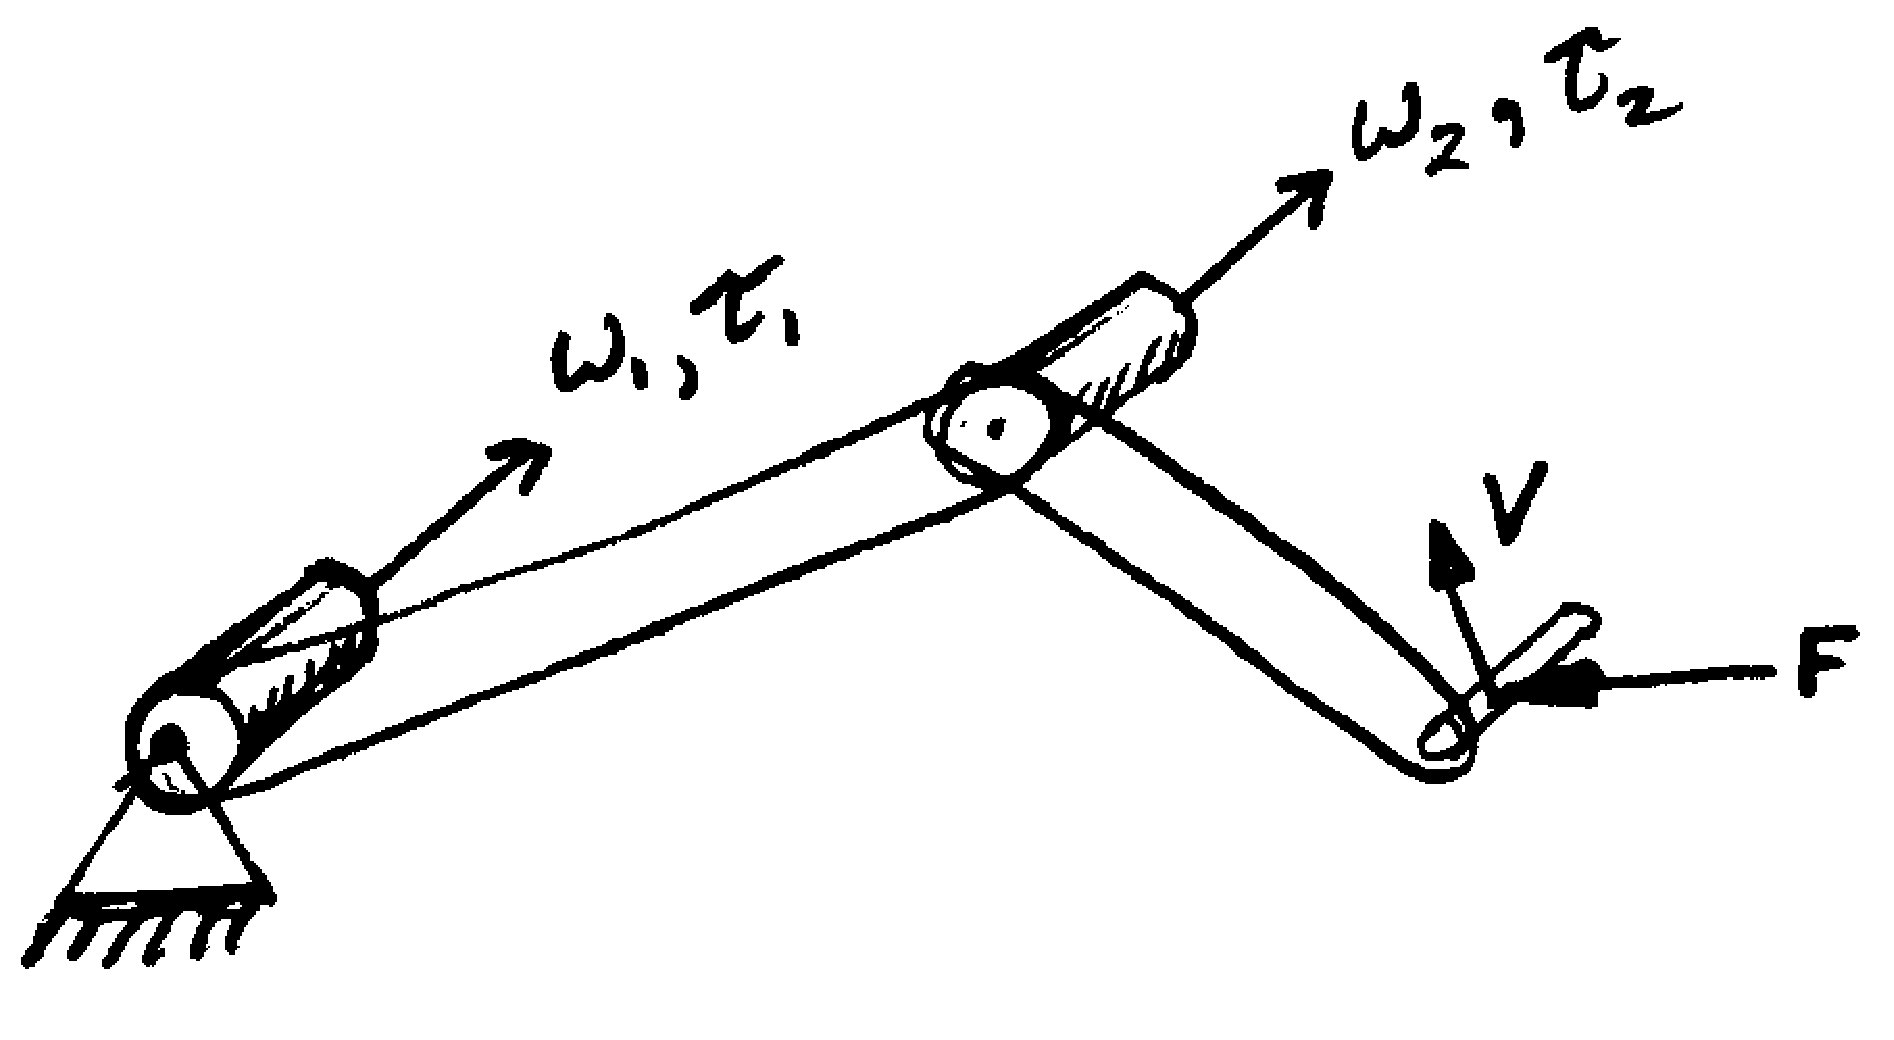
\includegraphics{figs05/00232.eps}
   }
\caption{Mechanism to illustrate Virtual Work.}\label{Crank}
\end{figure}

Let's consider a planar 2-link mechanism with a handle applied to the end (Figure \ref{Crank}).
If it helps, think of ideal generators attached to the joints which can extract energy from the joints.
If we crank on the
handle and compare the force and velocities of the handle with the joint torques and joint
angular velocities:
\[
F^TV = \tau^T \omega
\]
by the principle of Virtual Work.  If we multiply both sides by $\Delta t$,
\[
F^T\Delta X = \tau^T\Delta \Theta
\]
\[
\tau^T\Delta \Theta - F^T\Delta X = 0
\]
We know that
\[
\Delta X = J(\Theta) \Delta \Theta
\]
so
\[
\left( \tau^T - F^TJ \right ) \Delta \Theta = 0
\]
for finite $\Delta \Theta$:
\[
(\tau^T-F^TJ) = 0
\]
\[
\tau^T = F^T J
\]
\[
\tau = J^T F
\]
(because $(AB)^T = B^TA^T$ is a property of the matrix transpose).




%%%%** Section 3
\subsection{Velocity Propagation}

Now we investigate robot links arranged in a serial chain.  Remember that robot links are rigid bodies, and also
that adjacent robot links are rigidly joined or attached to each other {\it except} for motion
about/along the $Z_N$ axis.  For now, let's consider only rotary joints.


\begin{figure}\centering
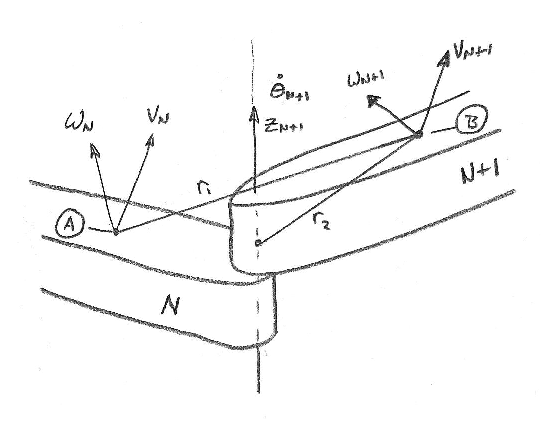
\includegraphics[width=85mm]{figs05/00611.eps}
\caption{Two links of a manipulator connected by a rotary joint.}\label{linkjointlink}
\end{figure}

Figure \ref{linkjointlink} shows two adjacent robot links.
For now, an arbitrary point is selected on
each link at which we define the linear and angular velocity for that link.
$r_1$ is a vector connecting the the defined points on two adjacent links.  $r_2$ is the unique
vector connecting the point on link $N+1$ to the origin of frame $N+1$.
Assume that all velocities are computed in the world frame,
$W$, and represented anywhere.

Then, assume they are a single rigid object (i.e. $\dot{\theta}_{N+1}=0$).
In that case, using the result above, we have
\[
\omega_{N+1} = \omega_N      \qquad     V_{N+1} = V_N + \omega_N\times r_1
\]

Now, assume that the joint velocity, $\dot{\theta}_{N+1} \ne 0$.  This adds a new component to both equations:


\[
\omega_{N+1} = \omega_N + Z_{N+1}\dot{\theta}_{N+1}     \qquad     V_{N+1} = V_N + \omega_N\times r_1 + \dot{\theta}_{N+1}Z_{N+1}\times r_2
\]

Finally, we can apply this to robot links and their DH parameters as follows:

\begin{enumerate}
  \item From our DH analysis, we know ${^N_{N+1}R},\; {^N_{N+1}T}$.
  \item Let point (A) be the origin of frame $N$, and point (B) be the origin of frame $N+1$
  \item In this case, $r_1 = [T_{14}, T_{24}, T_{34}]^T$ (the fourth column of ${^N_{N+1}T}$).
  \item Because (B) is the origin of frame $N+1$, $r_2 = 0$.
\end{enumerate}

Then, using known rotation matrix ${N+1}_NR$ to keep $^N\omega_N$ represented in its original frame, 
we get
 
\beq\label{angularvelocityprop}
^{N+1}\omega_{N+1} = \quad {^{N+1}_{N}R}\quad {^{N}\omega_{N}} +
\left[
\begin{array}{c}
0 \\
0 \\
\dot{\theta}_{N+1}
\end{array}
\right]
\eeq

and
\beq\label{linearvelocityprop}
^{N+1}V_{N+1} =\quad  {^{N+1}_{N}R}\left[
   ^{N}V_{N} +
   ^N\omega_{N} \otimes \quad ^NP_{N,N+1}
   \right]
\eeq

OK Professor, what have we accomplished? (because all the link linear and angular velocities ($^NV_N$, $^N\omega_N$) are still unknowns).   However, in fact initially $do$ know one pair:
\[
^0\omega_0 = 0 \quad \mathrm{and}  \quad ^0V_0 = 0
\] 
because the base of the robot is (hopefully) bolted down.   We also know
the joint velocities, $\dot\theta_N$ (from sensors for example), and the rotation matrices
$^{N+1}_NR$, and the link position offsets, $^NP_{N,N+1}$, from the forward kinematics.
Therefore, we can use equations \ref{angularvelocityprop} and \ref{linearvelocityprop} to compute each velocity one at a time.


\begin{ExampleSmall}
\paragraph{Derive similar equations for prismatic joints}

If we identify that joint $N+1$ is prismatic, then we replace the
above equations with the following.
A prismatic joint does not add {\it any} rotation, so
\[
^{N+1}\omega_{N+1} = \quad {^{N+1}_{N}R}\quad {^{N}\omega_{N}}
\]
but it does add a component of linear velocity in the $Z_{N+1}$ direction:
\[
^{N+1}V_{N+1} =\quad  {^{N+1}_{N}R}\left[
   ^{N}V_{N} +
   ^{N}\omega_{N} \otimes ^NP_{N,N+1}
   \right] +
\left[
\begin{array}{c}
0 \\
0 \\
\dot{d}_{N+1}
\end{array}
\right]
\]
\end{ExampleSmall}

Once the linear and angular velocities of the last link (end effector) of the manipulator are computed by this method of ``velocity propagation," it is a quick step to get the Jacobian matrix as illustrated by the following example:



\begin{Example}\label{JacobianExampleOne}
Compute the Jacobian Matrix by the Velocity Propogation method.  The manipulator is described by the following Denavit Hartenberg parameters:

\begin{center}
\begin{tabular}{|c|c|c|c|c|}
\hline
$i$	& $\alpha_{i-1}$	& $a_{i-1}$	& $d_i$		& $\theta_i$  \\ \hline
1	& 0			& 0		& 0		& $\theta_1$  \\ \hline
2	& $\pi/2$		& $L_1$		& 0		& $\theta_2$	\\ \hline
3	& 0			& $L_2$		& 0		& $\theta_3$	\\ \hline
4	& 0			& $L_3$		& 0		& 0		\\ \hline
\end{tabular}
\end{center}

\vspace{0.15in}
\textbf{Solution: }
First we need to generate the link transforms from the DH parameters, $^{i-1}_iT$
(hopefully we have them around from our forward kinematics step).

\[
^0_1T  =
\left [
\begin{array}{cccc}
c_1	& -s_1	& 0	& 0	\\
s_1	& c_1	& 0	& 0	\\
0	& 0	& 1	& 0	\\
0	& 0	& 0	& 1	\\
\end{array}
\right ]
\]
\[
^1_2T  =
\left [
\begin{array}{cccc}
c_2	& -s_2	& 0	& L_1	\\
0	& 0	& -1	& 0	\\
s_2	& c_2	& 0	& 0	\\
0	& 0	& 0	& 1	\\
\end{array}
\right ]
\]
\[
^2_3T  =
\left [
\begin{array}{cccc}
c_3	& -s_3	& 0	& L_2	\\
s_3	& c_3	& 0	& 0	\\
0	& 0	& 1	& 0	\\
0	& 0	& 0	& 1	\\
\end{array}
\right ]
\]
\[
^3_4T  =
\left [
\begin{array}{cccc}
1	& 0	& 0	& L_3	\\
0	& 1	& 0	& 0	\\
0	& 0	& 1	& 0	\\
0	& 0	& 0	& 1	\\
\end{array}
\right ]
\]

Now we propagate the angular velocities first (since they are needed for the linear step):

\[
^1\omega_1 =
\left[
\begin{array}{c}
0  \\ 0  \\ \dot{\theta_1}
\end{array}
\right ]
+
\begin{bmatrix}
0\\0\\0
\end{bmatrix}
\]

\[
^2\omega_2 =
\;^2_1R\;^1\omega_1 +
\left[
\begin{array}{c}
0  \\ 0  \\ \dot{\theta}_2
\end{array}
\right ]
\]
\[
=
\left [
\begin{array}{ccc}
c_2	& 0	& s_2	 	\\
-s_2	& 0	& c_2	 	\\
0	& -1	& 0	 	\\
\end{array}
\right ]
\left[
\begin{array}{c}
0  \\ 0 \\ \dot{\theta}_1
\end{array}
\right ]
+
\left[
\begin{array}{c}
0  \\ 0  \\ \dot{\theta}_2 \\
\end{array}
\right ]
\]

\[
^2\omega_2 =  \left[
\begin{array}{c}
s_2\dot{\theta}_1  \\ c_2\dot{\theta}_1 \\ \dot{\theta}_2
\end{array}
\right ]
\]

\[
^3\omega_3 =
\;^3_2R\;^2\omega_2 +
\left[
\begin{array}{c}
0  \\ 0  \\ \dot{\theta_3}
\end{array}
\right ]
\]

\[
=
\left [
\begin{array}{ccc}
c_3	& s_3	& 0		\\
-s_3	& c_3	& 0		\\
0	& 0	& 1		\\
\end{array}
\right ]
\left[
\begin{array}{c}
s_2\dot{\theta_1}  \\ c_2\dot{\theta_1} \\ \dot{\theta_2}
\end{array}
\right ]
+
\left[
\begin{array}{c}
0  \\ 0  \\ \dot{\theta_3} \\
\end{array}
\right ]
\]

\[
^3\omega_3 = \left[
\begin{array}{c}
s_2c_3\dot{\theta_1} + c_2s_3\dot{\theta_1}	\\
c_2c_3\dot{\theta_1} - s_2s_3\dot{\theta_1}	\\
\dot{\theta_2} + \dot{\theta_3}
\end{array}
\right]
=
\left[
\begin{array}{c}
s_{23}\dot{\theta_1} \\
c_{23}\dot{\theta_1} \\
\dot{\theta_2} + \dot{\theta_3}
\end{array}
\right]
\]



\[
^4\omega_4
= \; ^4_3R \; ^3\omega_3 +
\left[
\begin{array}{c}
0 \\0 \\ 0
\end{array}
\right ] = \; ^3\omega_3
\]





Now we propagate linear velocity using the previously calculated $^{i+1}_iT$ and $^i\omega_i$:

\[
^0V_0 =
\left[
\begin{array}{c}
0 \\0 \\ 0
\end{array}
\right ]
\]

\[
^1V_1 = \;^1_0R(^0V_0 + ^0\omega_0 \times \;^0P_1) =
\left[
\begin{array}{c}
0 \\0 \\ 0
\end{array}
\right ]
\]

\end{Example}
\begin{ExampleCont}

\[
^2V_2 = \;^2_1R(^1V_1 + ^1\omega_1 \times \;^1P_2) =
\]
\[
\left [
\begin{array}{ccc}
c_2	& 0	& s_2	 	\\
-s_2	& 0	& c_2	 	\\
0	& -1	& 0	 	\\
\end{array}
\right ]
\left[
\left[
\begin{array}{c}
0  \\ 0 \\ \dot{\theta_1}
\end{array}
\right ]
\times
\left[
\begin{array}{c}
L_1  \\ 0 \\ 0
\end{array}
\right ]
\right ]
\]

Here we can take advantage of the rule we identified in Section \ref{Rotation} and Section \ref{sectionrigidbodies}
in which the cross product can be represented as a skew symmetric matrix for faster computation.  In each stage of the linear velocity propagation, we will repeat the computation
\[
a\times b
\]
where $b = [L_i \quad 0 \quad 0]^T$.   For this case,
\[
a \times b =
\left[
\begin{array}{c}
0  \\[6pt] a_3L_i \\[6pt] -a_2L_i
\end{array}
\right ]
\]

Applying this we get
\[
^2V_2 =
\left [
\begin{array}{ccc}
c_2	& 0	& s_2	 	\\
-s_2	& 0	& c_2	 	\\
0	& -1	& 0	 	\\
\end{array}
\right ]
\left[
\begin{array}{c}
0  \\ L_1 \dot{\theta_1} \\ 0
\end{array}
\right ]
=
\left[
\begin{array}{c}
0  \\ 0 \\ -L_1 \dot{\theta_1}
\end{array}
\right ]
\]

%%%%%%%%%%%%%%%%%%%%%%%%%%%%                          3V3
\[
^3V_3 =
\left [
\begin{array}{ccc}
c_3	& s_3	& 0		\\
-s_3	& c_3	& 0		\\
0	& 0	& 1		\\
\end{array}
\right ]
\left[
\left[
\begin{array}{c}
0  \\ 0 \\ -\dot{\theta_1}L_1
\end{array}
\right ]
+
\left[
\begin{array}{c}
s_2\dot{\theta_1}  \\ c_2\dot{\theta_1} \\ \dot{\theta_2}
\end{array}
\right ]
\times
\left[
\begin{array}{c}
L_2  \\ 0 \\ 0
\end{array}
\right ]
\right ]
\]
\[
= \; ^3_2R
\left[
\begin{array}{c}
0 \\ \dot{\theta_2}L_2     \\   -(c_2L_2-L_1)\dot{\theta_1}
\end{array}
\right ]
\]
\[
^3V_3 =
\left[
\begin{array}{c}
s_3L_2\dot{\theta_2}  \\ c_3L_2\dot{\theta_2} \\  -(c_2L_2+L_1)\dot{\theta_1}
\end{array}
\right ]
\]

\vspace{0.15in}

%%%%%%%%%%%%%%%%%%%%%%%%%%%%%%5                      4V4
\[
^4V_4 =
\left [
\begin{array}{ccc}
1	& 0	& 0		\\
0	& 1	& 0		\\
0	& 0	& 1		\\
\end{array}
\right ]
\left[
^3V_3
+
\left[
\begin{array}{c}
s_{23}\dot{\theta_1} \\  c_{23}\dot{\theta_1} \\ \dot{\theta_2}+\dot{\theta_3}
\end{array}
\right ]
\times
\left[
\begin{array}{c}
L_3  \\ 0 \\ 0
\end{array}
\right ]
\right ]
\]
\[
^4V_4 =
\left[
\begin{array}{c}
s_3L_2\dot{\theta_2}   \\  (c_3L_2+L_3)\dot{\theta_2} + L_3\dot{\theta_3}  \\  -\dot{\theta_1}(L_1+c_2L_2+c_{23}L_3)
\end{array}
\right ]
\]

\end{ExampleCont}



\subsection{Jacobian Matrix from velocity expressions.}

Now that we have calculated angular and linear velocity of the end effector, we can create the Jacobian matrix by factoring out all of the $\dot{\theta}$ terms:

\[
\left[
\begin{array}{c}
\vspace{0.1in} \\ ^NV_N \\ \vspace{0.1in} \\\vspace{0.1in} \\ ^N\omega_N \\ \vspace{0.1in}\\
\end{array} \right ]_{6\times 1}
=
\left [
\begin{array}{ccc}
\vspace{0.1in} & & \\
& J & \\
\vspace{0.1in}& & \\
\end{array}\right]_{6\times N}
\left[
\begin{array}{c}
 \dot{\theta_1}   \\   \dot{\theta_2}  \\ \vspace{0.1in}\\ \dots \\ \vspace{0.1in} \\  \dot{\theta_N}
\end{array}
\right]_{N\times 1}
\]

\begin{ExampleCont}
% Applying this to Example 5.\ref{JacobianExampleOne},

\[
\left[
\begin{array}{c}
\vspace{0.1in} \\ ^4V_4 \\ \vspace{0.1in} \\\vspace{0.1in} \\ ^4\omega_4 \\ \vspace{0.1in}\\
\end{array} \right ]_{6\times 1}
=
\left [
\begin{array}{ccc}
\vspace{0.1in} & & \\
& J & \\
\vspace{0.1in}& & \\
\end{array}\right]_{6\times 4}
\left[
\begin{array}{c}
 \dot{\theta_1}   \\   \dot{\theta_2}  \\ \vspace{0.1in}\\ \dots \\ \vspace{0.1in} \\  \dot{\theta_4}=0
\end{array}
\right]_{4\times 1}
\]

\vspace{0.25in}

\[
^4J =  \left [
\begin{array}{ccc}
0		& s_3L_2	&	0	\\
0		& c_3L_2 + L_3 	& 	L_3	\\
-(L_1+C_2L_2+C_{23}L_3)	& 0	& 	0	\\
s_{23}		& 0		&	0	\\
c_{23}		& 0		& 	0	\\
0		& 1		&	1
\end{array} \right]
\]
Note that col 4 of the Jacobian is not defined because $\dot{\theta}_4=0$, but $L_3$ still matters. 
\end{ExampleCont}



\subsection{Jacobian Matrix by Differentiation}


\begin{figure}
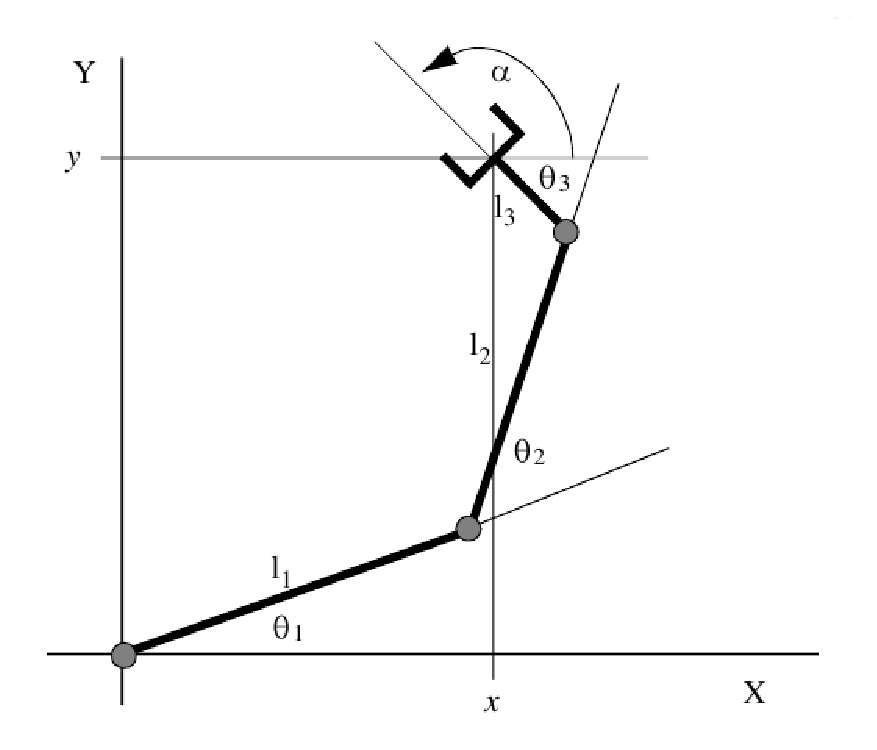
\includegraphics[width=3.5in]{figs05/planar_3link.eps}
\caption{3 Link planar manipulator.}\label{planar3link}
\end{figure}

In addition to the method of velocity propagation, the Jacobian matrix can also be obtained by differentiation of the forward kinematic equations.
Considering the 3-link planar manipulator of Figure \ref{planar3link}, define the configuration vector, $x = [x,y,\alpha]^T$.   The forward kinematic equations of this arm are:
\[
x = l_1c_1+l_2c_{12}+l_3c_{123} \qquad y =  l_1s_1+l_2s_{12}+l_3s_{123}  \qquad \alpha = \theta_1 + \theta_2+\theta_3
\]
Differentiating the first expression gives:
\[
\dot{x} = -l_1s_1\dot{\theta}_1-l_2s_{12}(\dot{\theta}_1+\dot{\theta}_2)-l_3s_{123}(\dot{\theta}_1+\dot{\theta}_2+\dot{\theta}_3)
\]
or
\[
\dot{x} = -(l_1s_1+l_2s_{12}+l_3s_{123})\dot{\theta}_1 - (l_2s_{12}+l_3s_{123})\dot{\theta}_2 - (l_3s_{123})\dot{\theta}_3
\]
Similarly,
\[
\dot{y} = (l_1c_1+l_2c_{12}+l_3c_{123})\dot{\theta}_1 - (l_2c_{12}+l_3c_{123})\dot{\theta}_2 - (l_3c_{123})\dot{\theta}_3
\]
and
\[
\dot{\alpha} = \dot{\theta}_1 + \dot{\theta}_2 + \dot{\theta}_3
\]
Thus,
\[
^0J{\theta} =
\left [ \begin{array}{ccc}
-l_1s_1-l_2s_{12}-l_3s_{123}    & -l_2s_{12}-l_3s_{123}  &  -l_3s_{123}   \\
l_1c_1+l_2c_{12}+l_3c_{123}     & l_2c_{12}+l_3c_{123}   & l_3c_{123}     \\
1 & 1 & 1
\end{array} \right ]
\]
Remember that we started with the expression for the end effector configuration in frame 0 so the resulting Jacobian is still in frame 0.  We have indicated this with a leading superscript above.   In contrast, the Jacobian computed by velocity propagation leaves us with a Jacobian in frame $N$ (we omitted the superscript in the examples above).  Both results are valid.  In general the Jacobian can be transformed into any desired frame as described in Section \ref{JacobianTransform}.


\begin{ExampleSmall}\label{ExJacob}

\includegraphics{figs04/00087.eps}

Compute the Jacobian matrix of the arm above where all three joints
$\theta_1, \dot{d}_2, \theta_3$ are variables.
Consider $\dot{x}, \dot{y},$ and the rate of change of
orientation of $x_4$, $\dot{\gamma}$. The Jacobian matrix
should have 3 rows.


Solution:


The forward kinematic equations are:

\[
x = d_{2}\cos\theta_{1}+ l_{3}\cos(\theta_1+\theta_3)
\]
\[
y = d_{2}\sin\theta_{1}+ l_{3}\sin(\theta_1+\theta_3)
\]
\[
\gamma=\theta_1+\theta_3
\]

Differentiating:

\[
\dot{x}= -d_{2}\sin\theta_1 \dot{\theta}_1
+\dot{d}_2\cos\theta_1
-l_{3}\sin(\theta_1+\theta_3)(\dot{\theta}_1+\dot{\theta}_3)
\]
\[
\dot{y}= d_{2}\cos\theta_1 \dot{\theta}_1
+\dot{d}_2\sin\theta_1
+l_{3}\cos(\theta_1+\theta_3)(\dot{\theta}_1+\dot{\theta}_3)
\]
\[
\dot{\gamma}=\dot{\theta}_1 + \dot{\theta}_2
\]

Factoring:

\[
J = \left[ \begin{array}{ccc}
-d_2s_1-l_3s_{13} & c_1 & -l_3s_{13} \\
d_2c_1+l_3c_{13} & s_1 & l_3c_{13} \\
1 & 0 & 1
\end{array}
\right]
\]
\end{ExampleSmall}




\section{Inverting the Jacobian Matrix}
We saw earlier that we will make frequent use of the Jacobian matrix for relating forces and velocities between the joints and the end effector spaces using the equations
\[
\dot{x} = J\dot{\theta}  \qquad  \tau = J^TF
\]
Just as with static kinematics of Chapter 2, these equations are often more useful if inverted.  Thus we frequently need a form such as
\[
\dot{\theta} = J^{-1}\dot{x}
\]
Computation of $J^{-1}$ is not a very time consuming job for today's processors.
As we have seen however, the elements of the Jacobian matrix are functions of the joint variables $\theta$ so if we use $J^{-1}$ we must compute it frequently as the manipulator moves around.  Since the numerical values of $J$ are always changing, we can't make a blanket statement about whether this inverse exists.  We often evaluate the ability to invert a matrix using its determinant.   In fact, in many practical robotic problems, there are configurations of the joints inside or throughout the workspace where
\[
\mathrm{Det}({J}) = 0
\]
and as a result, any computation, say inside a controller, which relies on a numerical method to find $J^{-1}$ will have problems.   The configurations of the joints of a manipulator at which $\mathrm{Det}({J}) = 0$ are called {\it singularities}.


\subsection{Interpretations of the Jacobian Inverse: Singularities}
Here we will look at some implications of basic linear algebra for the Jacobian Inverse.
We will make reference to some basic facts about matrices which are given in Appendix \ref{LinearAlgebraBasics}.

Consider the case of a square, 6x6, Jacobian matrix.  If rank$(J(\theta)) < 6$, then there is no solution to
\[
\dot{\theta} = J^{-1}(\theta)\dot{x}
\]
(see Facts 1 and 2).   Also,
by Fact 8, if the rank, $r=5$, there is one non-zero solution to
\[
\dot{x} = J(\theta)\dot{\theta} = 0
\]
The interpretation of this fact is that there is a direction in joint velocity space for which non-zero joint motion produces no end effector motion.
We call any joint configuration, $\theta = Q$ for which
\[
\mathrm{rank}(J(Q)) < 6
\]
a {\bf singular configuration}.

Furthermore, there are certain directions of end effector motion, $\dot{x}_i$, which are eigenvectors of $J(\theta)$. If $J$ is full rank, we have
\[
\dot{x}_i = J(\theta)\dot{\theta} = \lambda_i(\theta) \omega_i(\theta)
\]
where $\lambda_i$ are the eigenvalues of $J$ and $\omega_i$ are the eigenvectors of $J$. If $J$ is full rank, we have
\[
\omega_i = J^{-1}(\theta)\dot{x}_i = \lambda^{-1}_i\dot{x}_i
\]
(Fact 5).
As the manipulator approaches the singular configuration, $\theta \to Q$, there is at least one eigenvalue for which $\lambda_j \to 0$.  Thus
\[
\omega_j \to \frac{\dot{x}_j}{0} = \infty
\]

In words, as the manipulator approaches the singular configuration, motion in the particular direction $\dot{x}_j$ causes joint velocities to approach infinity.




\begin{ExampleSmall}\label{JacobianSingOne}
We will look at the specifics of singularities through an example, the planar 3-link manipulator of Figure \ref{planar3link}.   Let's look at Jacobian in the following configuration:
\[
Q = \left [ \begin{array}{c}
\pi/4 \\ 0 \\ \pi
\end{array} \right ]
\]
When the manipulator is posed such that $\theta = Q$, we have
\[
s_{12} = s_1 \qquad s_{123} = -s_1, \qquad c_{12} = c_1, \qquad c_{123} = -c_1
\]
This gives
\[
^0J(Q) = \begin{bmatrix}
(-l_1-l_2+l_3)s_1 & (-l_2+l_3)s_1  & l_3s_1        \\
(l_1+l_2-l_3)c_1  & (l_2-l_3)c_1   & -l_3c_1        \\
1 & 1 & 1
\end{bmatrix}
\]
If we denote the rows of $J$ by $\{r_1,r_2,r_3\}$, and recall that for $\theta_1=\pi/4$, then $s_1=c_1=0.707$, then we note that
\[
r_1 = -r_2
\]
and therefore det$[J(Q)]=0$ (Fact 3). This means that $Q$ is a singular configuration.  Note that on closer examination, we can see that $\theta_1$ does not have to be $\pi/4$ for this to happen.  This is because, for any $\theta_1$, we still have
\[
r1 = r2\times -\tan(\theta_1)
\]
$-\tan(\theta_1)$ is a constant which relates the two rows so that the matrix must be singular.   The proper way to describe the singular configuration is thus

\[
Q = \left [ \begin{array}{c}
\theta_1 \\ 0 \\ \pi
\end{array} \right ]
\]
for any $\theta_1$.

\end{ExampleSmall}



\begin{ExampleSmall}
Find any singular configurations of the manipulator of Example 5.\ref{ExJacob}
For each singular configuration:

1) Draw it and indicate which direction of motion
cannot be achieved.

2) State whether it is an
interior singularity or workspace boundary singularity.

\noindent
Use analysis of
the Jacobian to derive the result or confirm your graphical analysis.

Solution:

For $\theta_3 = 0$, $s_{13}=s_1$, $c_{13}= c_1$.
\[
J = \left[ \begin{array}{ccc}
-(d_2+l_3)s_{1} & c_1 & -l_3s_{1} \\
(d_2+l_3)c_{1} & s_1 & l_3c_{1} \\
1 & 0 & 1
\end{array}
\right]
\]
This is only singular when $d_2=0$, making two collumns equal.
% 
% \scalebox{1}{
%    \includegraphics{figs04/00090.eps}
%    }

 
\includegraphics[width=55mm]{figs05/01041a.eps}\\
Non singular pose: end point can move in all directions. 

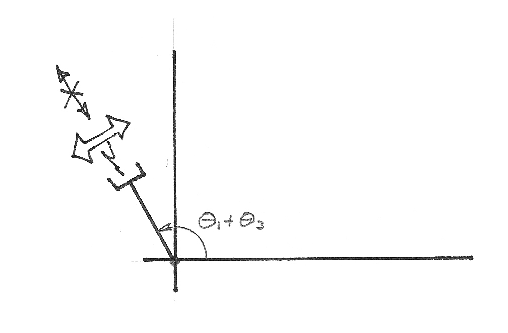
\includegraphics[width=55mm]{figs05/01041c.eps}\\
Singular pose where $d_2=0$.  Direction of blocked motion shown by thin arrow (crossed out).  Thick arrow shows direction in which motion is still possible. 

\includegraphics[width=55mm]{figs05/01041b.eps}\\
Pose where $\theta_3=\pi$.  Even though this ``looks" like a singular pose, 
in fact it is not since manipulator can still move in two directions.  



Note that there are no joint limits, infinite workspace, no
workspace boundary singularities.

\end{ExampleSmall}


\subsection{Force and torque at a kinematic singularity}
Since $\tau=J^T F$, at a singular point, $Q$, we can expect non-zero forces $F_j$ such that \[
J^T(Q)F_j = 0
\]
In words, there will be some force vector or vectors ($F_j$) which can be applied to the end effector, which generate no torques at the joints.  So, in a singular configuration, the mechanism can ``lock up" with respect to tip forces or torques in certain directions becuase these directions allow no torque to develop at the joints. For example, suppose $Q$ is defined as in Example \ref{JacobianSingOne} and
\[
F_1 = \begin{bmatrix} -F\cos\theta_1 \\ -F\sin\theta_1 \\ 0 \end{bmatrix}
\]
Note that this corresponds to a force applied to the tip in the direction opposite to the outstretched arm, and that no external torque is applied to the tip.  Now, writing $J^T(Q)$ in a simplified form:
\[
\tau = J^T(Q)F_1 =
\begin{bmatrix}
   as_1 & -ac_1 & 1  \\
   bs_1 & -bc_1 & 1  \\
   cs_1 & -cc_1 & 1  \\
\end{bmatrix}              =
\begin{bmatrix}
-Fc_1  \\ -Fs_1  \\ 0
\end{bmatrix}
\]
where $a = -l_1 -l_2 +l_3$, $b = -l_2 +l_3$, $c = l_3$.  And
\[
\tau = \begin{bmatrix}
-aFs_1c_1+aFs_1c_1 + 0 \\
-bFs_1c_1+bFs_1c_1 + 0   \\
0
\end{bmatrix}                 =
\begin{bmatrix}  0 \\ 0 \\ 0 \end{bmatrix}
\]
The end effector force is finite, but the torque on all joints is zero.
This situation is an old and famous one in mechanical engineering. For example, in an old railroad steam engine, ``top dead center" refers to the
state depicted in Figure \ref{TDC}.
The piston force, F, cannot generate any torque around the drive wheel axis because the linkage is in a singular configuration as shown.


\begin{figure}\centering
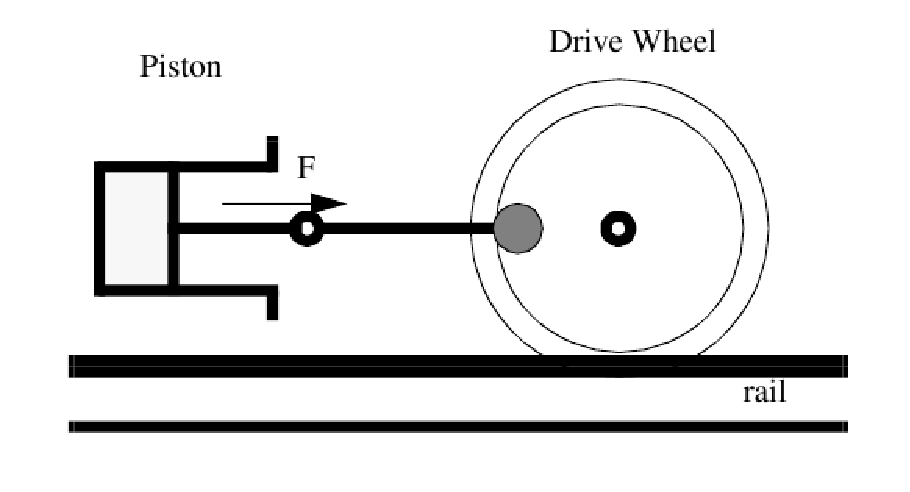
\includegraphics[width=3.5in]{figs05/top_dead_ctr.eps}
\caption{A piston from a steam locomotive in the ``Top-Dead-Center" position.}\label{TDC}
\end{figure}

\subsection{Velocity at a kinematic singularity}
Note that although in a singular configuration (i.e. certain ``poses" or values of 
$[\theta_1, \theta_2, \dots, \theta_i]^T$) $\dot{\theta}=J^{-1}(Q)\dot{x}$ has no solution in general, if we assume that $J$ looses rank by only one (i.e. $r-N=1$), then there are $N-1$ eigenvectors in the task velocity space, $\dot{x}_j$, for which solutions $do$ exist.  However, there will be multiple solutions.  For example, if
\[
\dot{x}_1 = \begin{bmatrix} -Vs_1 \\ Vc_1 \\ 0 \end{bmatrix}
\]

Assume the manipulator is posed as in Figure \ref{3linksingular}.  The velocity vector we have just described is also plotted in Figure \ref{3linksingular}.

\begin{figure}\centering
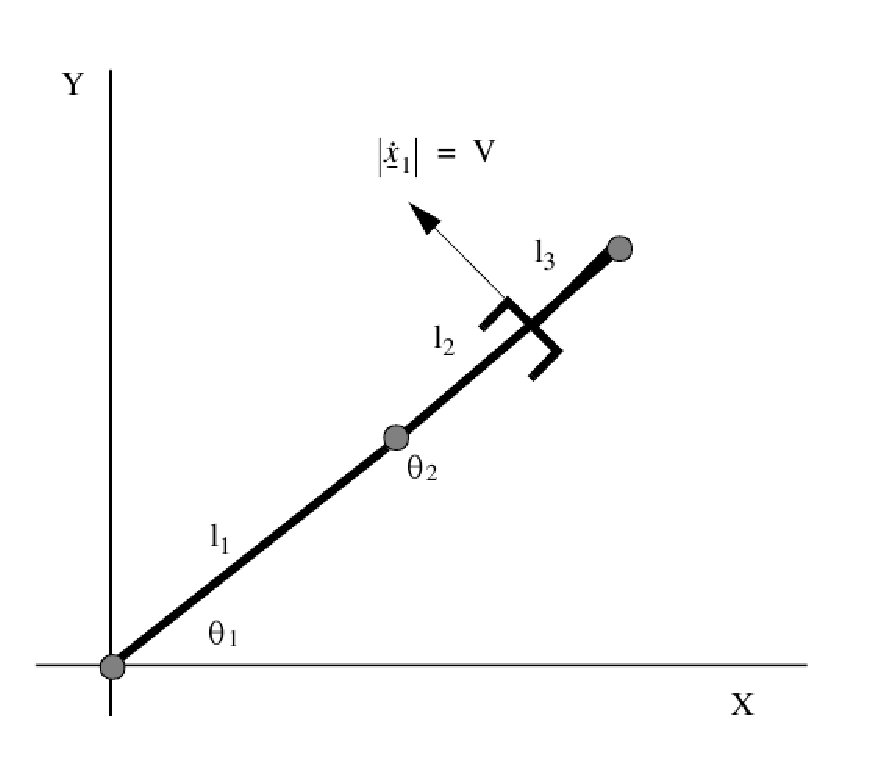
\includegraphics[width=3.5in]{figs05/sing1.eps}
\caption{A singular configuration of a 3 link manipulator.}\label{3linksingular}
\end{figure}

We can see (by looking at the lever arms between joints and the end effector) that the valid solutions for the resulting joint velocities will be

\[
\dot{\underline{\theta}}_1 = \begin{bmatrix} \frac{V}{(l_1+l_2-l_3)} \\ 0 \\ 0   \end{bmatrix}
\]
\[
\dot{\underline{\theta}}_2 = \begin{bmatrix} 0 \\ \frac{V}{(l_2-l_3)}   \\ 0   \end{bmatrix}
\]
\[
\dot{\underline{\theta}}_3 = \begin{bmatrix} 0 \\ 0 \\ \frac{V}{(-l_3)}    \end{bmatrix}
\]

where the underlined variable, $\underline{\dot{\theta}}_i$ is a vector of the individual joint velocities.
The end effector velocity is also satisified by  linear combinations of these solutions such as
\[
\underline{\dot{\theta}_n} = a_1\underline{\dot{\theta}}_1 +  a_2\underline{\dot{\theta}}_2 +  a_3\underline{\dot{\theta}}_3
\]
where $a_1+a_2+a_3=1$.    This can be verified by multiplying any of the solutions by $J(Q)$ to obtain $\dot{x}_1$.

However, if any component of the tip velocity in the direction corresponding to the zero eigenvalue of $J$ is non-zero, then at least one joint rate will go to infinity.



\subsection{Kinematic Conditioning}

So far we have looked at kinematic singularities from the point of view of specific joint values which cause the determinant to be zero.  For example, in Example \ref{JacobianSingOne}, when
\[
\theta = Q = \begin{bmatrix} \theta_1 \\ 0 \\ \pi \end{bmatrix}
\]
The manipulator was singular.  In practical cases and computational implementations however, we have to be concerned about situations where the manipulator is {\it almost} singular.    Suppose
\[
\theta = \begin{bmatrix} \theta_1 \\ 0.01 \\ 3.15 \end{bmatrix}
\]
Technically this is not singular.  However $J^{-1}$ may be difficult to compute.   A measure of this difficulty is the {\it condition number} of the Jacobian, designated $\kappa(J)$.   The condition number is
\[
\kappa(J) = \frac {\sigma_{max}(J)}  {\sigma_{min}(J)}
\]
where $\sigma_{max}$ is the maximum singular value $J$.  When the Jacobian matrix looses rank, at least one singular value becomes zero. As we approach the singualrity,  the condition number becomes very large.

As a practical matter, when using $J^{-1}$ in a computation, it is not the exact singular configurations which must be avoided, but rather the regions around and including the singular configurations where the condition number of $J$ exceeds a threshold.


\section{Transformation of Jacobian between Representation Frames}\label{JacobianTransform}

Recall that in both the velocity propagation and the differentiation methods, we computed a velocity first and then factored out $\dot{\theta}$ to create the Jacobian matrix.   Like any velocity, the one we base our Jacobian on could be represented in any frame and could be transformed by rotation between frames.  Factoring each of these representations of end effector velocity will thus give us a different Jacobian matrix.   The Jacobian matrix can thus be transformed among different frames by rotation as follows:

\[
^AJ(\theta) =
\begin{bmatrix}
 \begin{bmatrix}
     & & \\
     & {^A_BR} & \\
     & & \\
 \end{bmatrix}
&
 0  \\
 0 &
 \begin{bmatrix}
     & & \\
     & {^A_BR} & \\
     & & \\
 \end{bmatrix}
\end{bmatrix}
{^BJ(\theta)}
\]
The special $6\times6$ matrix contains two identical submatrices which are ${^A_BR}$.  These transform the linear and rotational components of the end-effector configuration space velocity separately but identically.  Importantly, since the above $6\times6$ matrix contains two orthonormal sub-matrices, the eigenvalues of $J$ are unchanged by this transformation.  Thus singularities and condition number are not changed by rotation of the Jacobian into different frames.




\section{Summary of Notation}

% Summary of Notation for Chapter  05

